\chapter{Quantum Error Correction and Fault Tolerance}
\lecture{19}{20 Nov. 10:30}{}  % L18이랑 통합
\section{Introduction}
Quantum noise는 universal quantum computer를 설계하기 위해 가장 중요하게 다뤄져야 하는 요소이다. Chapter 3에서는 quantum error를 표현하는 방법을 배웠고 이제 이 챕터에서는 quantum error를 정정하는 방법을 소개하려고 한다.

\section{Some distance measure}
Quantum noise로 인해서 state가 얼마나 많이 달라졌는지를 평가하기 위해서, \textit{distance measure}를 정의해야 한다. 이를 위해서 먼저 classical information에 대한 distance measure를 소개하고 이를 quantum information에 대해서 확장한 distance measure를 소개한다.
\subsection{Distance measures for classical information}
동일한 random variable $X$에 대해, 서로 다른 두 probability distribution $\{p_x\}$와 $\{q_x\}$를 가정하자. 이 두 distribution의 차이를 나타내기 위해 사용할 수 있는 한 가지 방법은 \textit{total variation distance (TVD)}이다:
\begin{equation*}
    D(p, q) \triangleq \frac{1}{2} \sum_{x}|p_x-q_x|
\end{equation*}
만약 두 분포가 동일하다면, TVD는 0이 된다. 반대로 두 분포가 \textit{orthogonal}하다면, TVD는 1이된다.\\
Total variation distance는 다음과 같은 성질을 가진다.
\begin{itemize}
    \item Symmetry: $D(p, q)=D(q, p)$
    \item Non-negativity: $D(p, q) \geq 0$
    \item Triangle inequality: $D(p, q) \leq D(p, r)+D(r, q)$
\end{itemize}
\vspace{1em}
반면, \textit{fidelity}를 사용하여 두 분포의 차이를 나타낼 수도 있다.
\begin{equation*}
    F\left(p_x, q_x\right) \triangleq \sum_x \sqrt{p_x q_x} 
\end{equation*}
마찬가지로 두 분포가 동일하다면, fidelity는 1이 되고 반대로 두 분포가 \textit{orthogonal}하다면 fidelity는 0이 된다. Fidelity 역시 0과 1사이의 값을 가지며 TVD와 반비례하는 값을 가진다.

(\textit{operational meaning}) TVD는 sample space의 가능한 모든 subset $S$에 대해서 두 분포의 차이가 최대가 되게하는 $S$의 space에 대한 TVD와 동일한 값을 가진다.
\begin{equation*}
    D(p, q)=\max _S|p(S)-q(S)|=\max _S\left|\sum_{x \in S} p_x-\sum_{x \in S} q_x\right|,
\end{equation*}


\subsection{Trace distance}
Trace distance는 TVD를 quantum distance measure로 확장한 것이다.\footnote{quantum density matrix에서 대��성분은 확률을 의미 한다.} ($|A| \triangleq \sqrt{A^\dagger A}$)
\begin{equation*}
    D(\rho, \sigma) \equiv \frac{1}{2} \operatorname{Tr}[|\rho-\sigma|],
\end{equation*}
Trace distance가 가지는 중요한 성질중에 하나는 바로 unitary operation에 대해서 invariant하다는 것이다.
\begin{equation*}
    D(\rho, \sigma)=D(U\rho U^\dagger, U\sigma U^\dagger)
\end{equation*}
Trace distance는 다음과 같이 나타낼 수도 있으며, 이는 가능한 모든 POVM set에 대해서 두 trace의 차이가 최대가 되도록 하는 POVM에 대한 trace distance로 정의할 수 있음을 의미한다. (TVD의 두 번째 정의)
\begin{equation*}
    D(\rho, \sigma)=\max _{\left\{M_x\right\}}\left|\operatorname{Tr}\left[M_x \rho\right]-\operatorname{Tr}\left[M_x \sigma\right]\right|,
\end{equation*}
Trace distance에 대해 중요한 특징이 존재하는데 이는 동일한 trace preserving quantum operator를 가했을 때, trace distance는 \textit{증가할 수 없다}는 정리이다.
\begin{equation*}
    D(\mathcal{E}(\rho), \mathcal{E}(\sigma)) \leq D(\rho, \sigma) 
\end{equation*}

\subsection{Quantum fidelity} \label{sec:quantum-fidelity}
다음으로 살펴볼 Quantum fidelity는 fidelity를 quantum distance measure로 확장한 것이다.
\begin{equation*}
    F(\rho, \sigma) \triangleq \operatorname{Tr} \sqrt{\sqrt{\rho} \sigma \sqrt{\rho}}
\end{equation*}
Quantum fidelity는 trace distance와 유사하게 다음과 같은 성질을 가진다.
\begin{itemize}
    \item Symmetry: $F(\rho, \sigma)=F(\sigma, \rho)$
    \item Invariant of unitary: $F(\rho, \sigma)=F(U\rho U^\dagger, U\sigma U^\dagger)$
    \item Operation inequality: $F(\mathcal{E}(\rho), \mathcal{E}(\sigma)) \geq F(\rho, \sigma)$
\end{itemize}

만약, $\rho=\sum_i r_i|i\rangle\langle i|, \sigma=\sum_i s_i|i\rangle\langle i|$가 commute하다면 quantum fidelity는 classical fidelity와 같다.
\begin{equation*}
    F(\rho, \sigma)=\operatorname{Tr}\left[\sqrt{\sum_i r_i s_i|i\rangle\langle i|}\right]=\sum_i \sqrt{r_i s_i}=F\left(r_i, s_i\right)
\end{equation*}
또한, 만약 두 state중에서 적어도 하나가 pure state라면, quantum fidelity는 다음과 같이 나타낼 수 있다.\footnote{계산이 간단하다.}
\begin{equation*}
    F(|\psi\rangle, \rho)=\operatorname{Tr}[\sqrt{\langle\psi| \rho|\psi\rangle|\psi\rangle\langle\psi|}]=\sqrt{\langle\psi| \rho|\psi\rangle} .
\end{equation*}

Quantum fidelity의 중요한 정의는 Uhlmann's theorem에 의해 주어진다. 이 정리는 양자 상태 사이의 fidelity를 pure state들의 overlap으로 생각할 수 있음을 주장한다.
\begin{theorem}[Uhlmann's theorem]
    $\rho$와 $\sigma$가 quantum system $Q$의 state일 때, quantum system $Q$의 복사본인 다른 system $R$에 대해 다음이 만족한다.
    $$ F(\rho, \sigma)=\max _{|\psi\rangle,|\varphi\rangle}|\langle\psi | \varphi\rangle| $$
    $\ket \psi, \ket \varphi$는 $\rho$, $\sigma$에 대해 $RQ$로 purification하여 나타낸 가능한 모든 pure state이다.
\end{theorem}

Quantum fidelity는 가능한 모든 POVM에 대한 classical fidelity를 사용하여 정의할 수 있다.
\begin{equation*}
    F(\rho, \sigma)=\min_{\{\Pi_m\}} F\left(p_m, q_m\right)
\end{equation*}

마지막으로, trace distance와 fidelity는 다음과 같은 관계를 만족한다.
\begin{equation*}
    1-F(\rho, \sigma) \leq D(\rho, \sigma) \leq \sqrt{1-F(\rho, \sigma)^2} .
\end{equation*}

\section{The basic code and Shor code}
\subsection{Classical error correction}
\begin{figure}
    \centering
    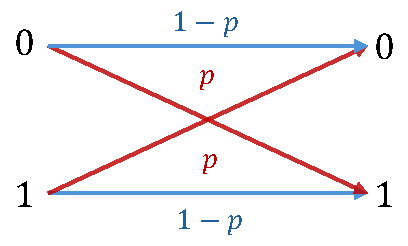
\includegraphics[width=0.3\textwidth]{figures/classical-bit-flip.pdf}
    \caption{Classical bit flip}
    \label{fig:bit-flip}
\end{figure}

Classical channel에서 발생할 수 있는 가장 간단한 오류인 bit flip error를 생각해보자. 아무런 인코딩도 하��� 않는다면 수신자의 입장에서 bit 1을 받았을 때 원래 1인지 아니면 0이었는데 bit flip error가 발생한 것인지를 구분할 수 없다.
이를 해결하기 위해 $0$이나 $1$대신에 비트를 반복해서 $000$, $111$으로 인코딩하여 bit flip error를 해결할 수 있다. 만약 오류의 발생확률 $p$가 충분히 작다면 오류가 발생한 bit string이 $001$일 때 $000 \rightarrow 001$의 확률이 $111 \rightarrow 001$의 확률보다 작다는 사실을 이용하여 오류 정정을 할 수 있다. 

\textit{Repetition code}의 성공 확률은 오류가 발생하지 않을 확률과 하나의 단일 비트에만 오류가 발생했을 확률의 합이며,
\begin{equation*}
    (1-p)^3+3p(1-p)^2 = 1 + 2p^3 - 3p^2
\end{equation*}
실패 확률은 2개의 이상의 비트에 오류가 발생했을 확률이다.
\begin{equation*}
    P_e  = 3p^2(1-p) + p^3 = - 2p^3 + 3p^2 
\end{equation*}
그렇다면, 오류 확률 $p$가 얼마나 작을 때 오류 정정 코드를 사용하는 것이 유리한지를 오류 정정을 하지 않았을 때의 실패 확률 $p$와 비교하여 계산할 수 있다.
\begin{equation*}
    p_e = -2p^3 + 3p^2 < p \quad \rightarrow \quad p < \frac{1}{2}
\end{equation*}

\subsection{The three qubit bit flip code}
Classical communication에서 이미 검증된 repetition code를 quantum communication에 바로 적용할 수 없는 이유는 다음과 같다.
\begin{itemize}
    \item No cloning : 주어진 임의의 양자상태를 복사할 수 없으므로 repetition이 불가능하다.
    \item Continuous error : 양자 채널은 bit flip error말고도 다른 다양한 오류가 존재한다.
    \item Measurement : 오류 정정을 위해서 state를 확인하면 기존의 quantum state가 붕괴된다.
\end{itemize} 
지금부터는 이러한 문제들을 어떤 방식을 도입하여 해결하였는지 소개하려고 한다. 먼저, $\ket \psi$에 $p$의 확률로 $X$ gate가 작용하여 state가 $X \ket \psi$로 변하는 bit flip error에 대해서만 생각해보자.
이를 해결하기 위해서 $\ket{0_L}, \ket{1_L}$을 physical qubit 3개로 표현되는 logical qubit으로 인코딩하자. \footnote{두 state $\ket 0, \ket 1$은 서로 orthogonal state이므로 복사할 수 있다.}
\begin{equation*}
    a|0\rangle+b|1\rangle \rightarrow a|000\rangle+b|111\rangle \equiv a\left|0_L\right\rangle+b\left|1_L\right\rangle,
\end{equation*}

그러나, logical qubit을 사용하더라도 여전히 오류가 발생했는지 확인하기 위해서 중간에 상태를 관측하면 기존의 정보를 모두 잃어버리게 되므로 \textbf{state를 관측하지 않고도 오류의 발생을 감지할 수 있는} 다른 방법이 필요하다.
이를 위해서 \textit{Syndrome measurement}를 제안한다. 
\begin{itemize}
    \item $P_0 = |000\rangle\langle 000| + |111\rangle\langle 111|$ : 오류가 발생하지 않음
    \item $P_1 = |100\rangle\langle 100| + |011\rangle\langle 011|$ : 첫 번째 qubit에 bit flip이 발생함
    \item $P_2 = |010\rangle\langle 010| + |101\rangle\langle 101|$ : 두 번째 qubit에 bit flip이 발생함
    \item $P_3 = |001\rangle\langle 001| + |110\rangle\langle 110|$ : 세 번째 qubit에 bit flip이 발생함
\end{itemize}

이 syndrome measurement set을 사용하면, 발생할 수 있는 모든 오류\footnote{여기서는 single bit flip error만을 커버한다.}들의 subspace에 projection 시키기 때문에 측정 후에도 quantum state의 정보는 그대로 유지된다. 
\begin{equation*}
    \frac{P_0 \ket \psi}{\langle \psi | P_0^\dagger P_0 | \psi \rangle } = \frac{a|000\rangle + b |111\rangle}{a\langle 000|+ b\langle 111| ( |000\rangle\langle 000| + |111\rangle\langle 111| )a|000\rangle+b|111\rangle} = \frac{a|000\rangle + b|111\rangle}{a^2 + b^2} = \ket \psi
\end{equation*}
Syndrome measurement set을 사용해서 얻은 outcome을 확인하면, 어떤 qubit에 bit flip이 발생하였는지 알 수 있고 그 qubit에 $X$ gate를 가하여 오류를 정정할 수 있다. 

\vspace{1em}

Quantum repetition code의 실패 확률 역시 classical repetition code와 동일하게 $P_e = - 2p^3 + 3p^2$이며, $p < 1/2$일 때 오류 정정을 하지 않을 때보다 더 정확도가 증가한다. 그러나 quantum bit flip error는 classical bit flip error처럼 단순하게 실패 확률을 분석해서는 안된다.
예를 들어, 오류가 발생하기 전 상태가 $\ket +$였다면, bit flip error는 아무런 영향을 주지 못하기 때문이다. 따라서 \textit{state distance}의 관점에서 오류를 분석할 필요가 있다. (오류가 없는 이상적인 상태는 항상 pure state이므로 \textit{fidelity}를 $F = \sqrt{\langle \psi | \rho | \psi \rangle}$로 쉽게 계산할 수 있으므로 fidelity를 사용하자.)

Quantum error correction의 목표는 \hyperref[sec:quantum-fidelity]{fidelity}를 증가시키는 것이다.\footnote{두 상태가 유사할수록 fidelity가 증가한다.}  만약 오류 정정을 하지 않는다면, output state는 다음과 같이 표현된다.
\begin{equation*}
    \rho=(1-p)|\psi\rangle\langle\psi|+p X|\psi\rangle\langle\psi| X .
\end{equation*}
따라서 두 상태간의 fidelity는 다음과 같이 ���산된다. 주어진 항에서 $\langle \psi | X | \psi \rangle$는 확률을 나타내는 값이므로 음수가 될 수 없다. $\ket \psi$가 computational state일 때, $\langle \psi | X | \psi \rangle = 0$이므로 minimum fidelity는 $\sqrt{1-p}$이라는 사실을 알 수 있다.
\begin{equation}
    F(\ket \psi \bra \psi, \rho)=\sqrt{\langle\psi| \rho|\psi\rangle}=\sqrt{(1-p)+p\langle\psi| X|\psi\rangle\langle\psi| X|\psi\rangle} \label{eq:fidelity-1}
\end{equation}
반면, 오류 정정을 수행했다면 1 bit flip error가 발생했더라도 오류정정을 통해 pure state를 그대로 유지할 수 있으므로 output state는 다음과 같고 
\begin{equation*}
    \rho_{QEC}=\left[(1-p)^3+3 p(1-p)^2\right]|\psi\rangle\langle\psi| + positive\ terms\ \cdots
\end{equation*}
fidelity는 다음의 lower bound를 가진다.
\begin{equation}
    F(\ket \psi \bra \psi, \rho_{QEC})  = \sqrt{(1-p)^3+3 p(1-p)^2 + positive\ terms\ \cdots}  \ge \sqrt{(1-p)^3+3 p(1-p)^2} \label{eq:fidelity-2}
\end{equation}
Eq.~\eqref{eq:fidelity-1}보다 Eq.~\eqref{eq:fidelity-2}의 값이 더 커지게 만들기 위해서는 $p < 1/2$여야 한다.

\vspace{1em}

Syndrome measurement를 이해하는 한 가지 다른 방법이 있다. 앞에서 제안한 4개의 projector를 사��하는 대신 2개의 observable을 측정한다고 생각해보자. 첫 번째로 $Z_1Z_2$\footnote{$Z_1Z_2 \triangleq  +\left((|00\rangle\langle 00|+|11\rangle\langle 11|)_{12} \otimes I_3\right) - \left((|01\rangle\langle 01|+|10\rangle\langle 10|)_{12} \otimes I_3 \right)$}를 측정하고
\begin{equation*}
    (Z_1Z_2) \qquad +1:(|00\rangle\langle 00|+|11\rangle\langle 11|)_{12} \otimes I_3, \quad-1:(|01\rangle\langle 01|+|10\rangle\langle 10|)_{12} \otimes I_3
\end{equation*}
이후 $Z_2Z_3$을 측정한다. 각각의 observable을 측정했을 때, $-1$이라는 outcome을 얻으면 해당 bit들의 값이 다르다는 것을 의미한다. 예를 들어 $Z_1Z_2$의 outcome이 $-1$이라면 첫 번째, 두 번째 qubit의 값이 다르다는 의미이다.
따라서 2개의 observable을 측정하여 얻은 outcome을 사용하여 어떤 qubit에 bit error가 발생하였는지를 추측하고 오류 정정을 수행할 수 있다. 


\begin{figure}[h]
    \begin{subfigure}[b]{0.5\textwidth}
        \centering
        \[
            \begin{array}{c}
            \Qcircuit @C=0.9em @R=1.6em {
                \lstick{\ket{\psi}} & \qw & \ctrl{1} & \ctrl{2} & \qw \\
                \lstick{\ket{0}} & \qw & \targ & \qw & \qw \\
                \lstick{\ket{0}} & \qw & \qw & \targ & \qw \\
            }
            \end{array}
            \]
        \caption{Three-qubit repetition code} \label{fig:repitition-circuit}
    \end{subfigure}
    \begin{subfigure}[b]{0.5\textwidth}
        \centering
        \[
            \begin{array}{c}
            \Qcircuit @C=1.0em @R=1.4em {
                \lstick{\ket{\psi}} & \qw & \ctrl{1} & \ctrl{2} & \gate{H} & \qw \\
                \lstick{\ket{0}} & \qw & \targ & \qw & \gate{H} & \qw \\
                \lstick{\ket{0}} & \qw & \qw & \targ & \gate{H} & \qw \\
            }
            \end{array}
            \]
        \caption{Three-qubit phase flip code} \label{fig:phse-flip-circuit}
    \end{subfigure}
    \caption{Three-qubit encoding circuits}
\end{figure}


\subsection{The three qubit phase flip code}
이번에는 phase flip error; $Z$ error에 대해 생각해보자. $Z$ error의 정정 역시 $X$ error의 정정과 동일한 방식을 도입하여 해결할 수 있다. Computational basis(X-basis) 대신에 Z-basis를 사용하여 state를 인코딩하며 syndrome measurement set을 사용하여 오류를 감지하고 오류가 발생한 qubit에 $Z$ gate를 가함으로서 phase flip error를 쉽게 해결할 수 있다. 
\begin{equation*}
    \left|0_L\right\rangle \equiv|+++\rangle, \quad\left|1_L\right\rangle \equiv|---\rangle .
\end{equation*}

\subsection{The Shor code}
지금까지 소개한 방식은 특정한 type의 single-qubit error만 해결할 수 있는 방법이다. 그렇다면, 다양한 single qubit error를 한번에 정정할 수 있는 방법은 없을까? Shor code가 바로 \textit{arbitrary single qubit error}를 모두 정정할 수 있는 방법이다. Shor code는 three qubit phase flip code와 bit flip code를 함께 적용한 간단한 방식을 사용한다.
\begin{enumerate}
    \item Encode the qubit using \textit{phase flip code}:
    \begin{equation*}
        |0\rangle \rightarrow|+++\rangle, \quad|1\rangle \rightarrow|---\rangle
    \end{equation*}
    \item Encoding each of the qubits \textit{bit flip code}:
    \begin{equation*}
        |+ \rangle = \frac{\ket 0 + \ket 1}{\sqrt 2} \rightarrow \frac{\ket{000} + \ket{111}}{\sqrt 2}, \quad |-\rangle = \frac{\ket 0 - \ket 1}{\sqrt 2} \rightarrow \frac{\ket{000} - \ket{111}}{\sqrt 2}
    \end{equation*}
\end{enumerate}
따라서 위의 인코딩 과정을 거치면 1개의 logical qubit은 \textbf{9개}의 physical qubit으로 구현된다. 
\begin{align*}
    |0\rangle \rightarrow\left|0_L\right\rangle & \triangleq \frac{(|000\rangle+|111\rangle)(|000\rangle+|111\rangle)(|000\rangle+|111\rangle)}{2 \sqrt{2}} \\
    |1\rangle \rightarrow\left|1_L\right\rangle & \triangleq \frac{(|000\rangle-|111\rangle)(|000\rangle-|111\rangle)(|000\rangle-|111\rangle)}{2 \sqrt{2}}
\end{align*}

이제 Shor code가 어뗳게 single qubit error를 정정할 수 있는지 살펴보자. 만약 $q_1$에 bit flip error가 발생했다면 observable $Z_1Z_2, Z_2Z_3$의 측정 결과로부터 $q_1$에 오류가 발생했다는 것을 알 수 있고 $X$ gate를 가하여 오류를 해결할 수 있다. 이처럼 Shor code는 bit flip error를 해결할 수 있다.
다음으로 $q_1$에 phase flip error가 발생했다고 하자. Phase flip은 computational basis에 대해서 qubit의 부호를 반전시키므로 $\ket{000} + \ket{111}$이었던 첫 번째 블록이 $\ket{000} - \ket{111}$으로 바뀌게 된다. 이 오류를 감지하기 위해서 우리는 각 블록($\ket{q_1q_2q_3}$)의 부호를 비교할 수 있도록 syndrome measurement를 사용할 수 있다. 
측정 결과로 첫 번째 블록과 두 번째 블록의 부호가 다르고 두 번째 블록과 세 번째 블록의 부호가 동일하다는 정보를 알게 되면, 첫 번째 블록 안의 어떤 qubit에서 phase flip이 발생했다고 추정할 수 있기 때문에 첫 번째 블록에 속한 qubit에 $Z$ gate를 가하�� phase flip error도 해결할 수 있다. Phase flip error를 감지하기 위해 사용하는 syndrome measurement는 다음과 같다.
\begin{equation*}
    X_1X_2X_3X_4X_5X_6, \quad X_4X_5X_6X_7X_8X_9
\end{equation*}
그렇다면 $q_1$에 bit flip error와 phase flip error가 동시에 발생했을 때는 어떻게 될까? 이 경우에는 단순히 bit flip error를 정정하는 단계와 phase flip error를 정정하는 단계를 모두 수행하여 문제를 해결할 수 있다.

이제 마지막으로, Shor code가 \textit{arbitrary single qubit error}를 정정할 수 있음을 보이고자 한다. 흥미롭게도, arbitrary single qubit error를 정정하는 과정 또한, 앞에서 설명했던 bit flip error와 phase flip error를 정정하는 두 방법을 적용하는 것으로 쉽게 해결할 수 있다.
이는 단일 큐빗에서 발생할 수 있는 \textbf{연속적인} 오류를 정해진 discrete subset of errors (i.e., X, Z, XZ)을 정정함으로써 모두 해결할 수 있다는 것을 의미한다.
이것이 왜 가능한 걸까? 첫 번째 qubit에 arbitrary single qubit error가 발생했다고 하자. 이 오류는 Kraus operator $\{E_i\}$를 사용하여 다음과 같이 표현될 수 있다.
\begin{equation*}
    \mathcal{E}(|\psi\rangle\langle\psi|)=\sum_i E_i|\psi\rangle\langle\psi| E_i^{\dagger}
\end{equation*}
전체 오류 대신, 합의 각 항 $E_i | \psi \rangle \langle \psi | E_i^\dagger$에 대한 정정을 생각해보자. 
우리는 어떤 single qubit operator도 다음과 같이 Pauli operator의 linear combination으로 표현할 수 있다는 사실을 알고있다.\footnote{$Y= XZ$}
\begin{equation*}
    E_i = e_{i0} I + e_{i1} X_1 + e_{i2} Z_1 + e_{i3} X_1Z_1
\end{equation*}
따라서 이 operator가 pure state $\ket \psi$에 작용한다면, 다음 4개의 항의 superposition 상태가 될 것이다.
\begin{equation*}
    |\psi\rangle, \quad X_1|\psi\rangle, \quad Z_1|\psi\rangle, \quad X_1 Z_1|\psi\rangle 
\end{equation*}
Shor code에서 사용하는 syndrome measurement는 $I, X, Z, XZ$가 가해졌을 때 얻을 수 있는 error들의 subspace로 \textit{projection}시키는 역할을 수행하기 때문에, syndrome measurement를 가하면 error state들의 superposition state가 붕괴해서 하나의 state가 된다.
각각의 상태는 Shor code의 오류 정정 과정을 사용할 수 있으므로(apply X, Z, XZ), 최종적으로 오류가 정정된 state로 변하게 된다. 
이것이 바로 Shor code가 arbitrary single qubit error를 정정할 수 있는 이유이다.

\begin{figure}[h]
    \centering
    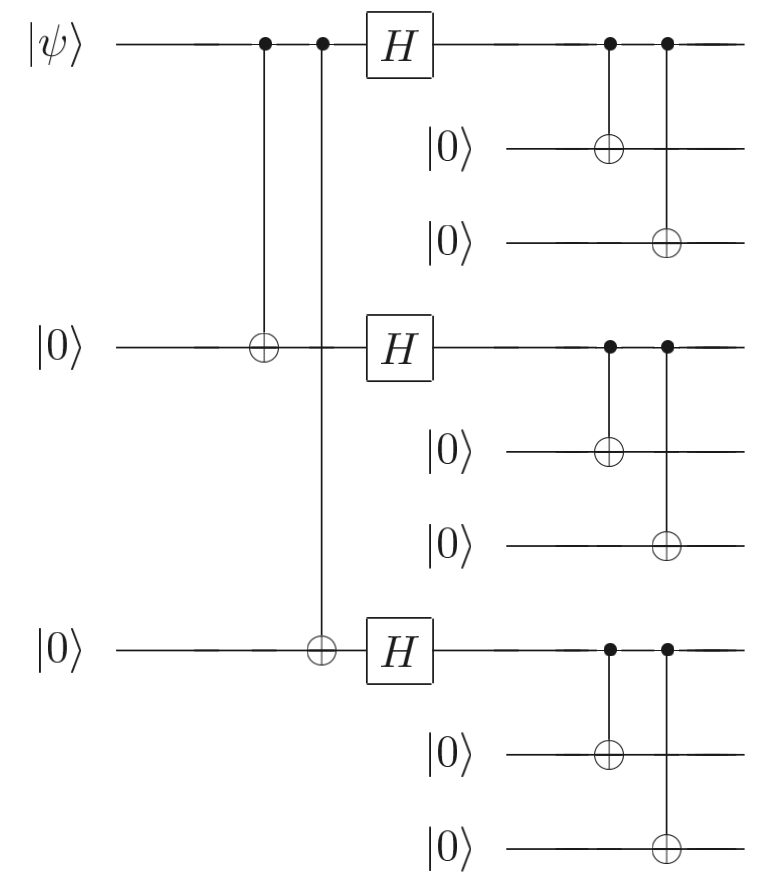
\includegraphics[width=0.4\textwidth]{figures/Shor_code.png}
    \caption{Shor code circuit} \label{fig:Shor-circuit}
\end{figure}

\lecture{20}{25 Nov. 10:30}{}
\section{Theory of QEC}
이전 섹션에서 우리는 Shor code를 통하여 arbitrary single qubit error를 정정할 수 있음을 보였다. 그렇다면 여러 bit에 동시에 error가 발생하는 경우에도 오류 정정을 수행할 수 있을까? 더 나아가, Quantum error correction(QEC)와 관련된 일반적인 이론을 정립할 수 있을까?
이 섹션에서는 QEC를 다루기 위해 사용하는 기초적인 툴에 대해서 소개하고, QEC가 가능하기 위한 조건에 대해서 살펴보고자 한다.

\vspace{1em}
기본적인 아이디어는 Shor code에서 도입한 개념을 일반화 하는 것이다. 양자 상태(i.e., physical qubit)는 unitary operator를 통해서 오류 정정 코드(i.e., logical qubit)로 인코딩된다. 오류 정정 코드는 기존 양자 상태보다 더 큰 Hilbert space의 subspace $C$로 정의된다.\footnote{예를 들어, 3-qubit repetition code에서 오류 정정 코드가 사용하는 vector space $C$는 span$\{\ket{000}, \ket{111}\}$} $C$에 대한 projector는 $P$로 나타낸다. 예를 들어, three qubit  bit flip code의 projector는 다음과 같다.
\begin{equation*}
    P=|000\rangle\langle 000|+|111\rangle\langle 111| 
\end{equation*}
인코딩 이후 코드는 noisy channel을 통과하면서 noise에 영향을 받게 되고 이후 syndrome measurement를 수행한다. Syndrome measurement를 수행하여 어떤 종류의 오류가 발생하였는지 확인하여 \textit{error syndrome}을 결정한다. Error syndrome을 확인한 뒤 \textit{recovery operation}이 수행되어 다시 original state로 복원된다.

이러한 아이디어를 시각적으로 보여주는 것이 바로 Fig.~\ref{fig:code-space}이다. 왼쪽에 있는 정육면체가 바로 original state의 subspace를 의미한다. 이 vector space안에 있는 original state에 서로 다른 종류의 error가 발생하면 오른쪽의 그림처럼 $A_1, A_2, \cdots A_6$의 서로다른 vector space로 vector space가 변하게 된다.
이때 (B)는 error subspace들이 서로 disjoint하기 때문에 noise channel을 통과한 후 state가 어떤 subspace에 위치하는지를 판단한 뒤 쉽게 오류 정정이 가능하다. 그러나, (A)의 경우에는 서로 다른 error subspace간에 겹치는 부분이 발생하기 때문에 \textbf{모호성}이 존재하게 된다.

\begin{figure}
    \centering
    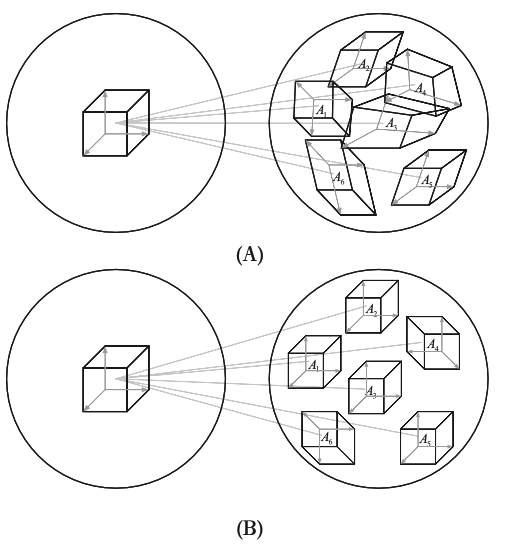
\includegraphics[width=0.4\textwidth]{figures/code_space.png}
    \caption{Code space} \label{fig:code-space}
\end{figure}

따라서 QEC가 가능하려��� 각각의 \textit{error syndrome}이 original Hilbert space의 \textbf{undeformed} and \textbf{orthogonal} subspace를 나타내야한다.

\vspace{1em}

QEC의 general theory를 정립하기 위해서는 noise와 오류 정정 과정에 대해서 최대한 적은 가정을 해야한다. 예를 들어 Shor code가 사용했던 가정들인 QEC가 detection \& recovery의 phase로 이루어지고 error가 특정한 qubit에만 발생하며 error 발생 확률 $p$는 충분히 작다와 같은 가정을 하지 않는다.
대신에 우리는 다음의 2가지 가정만을 사용한다.
\begin{itemize}
    \item Quantum noise는 quantum operation $\mathcal E$로 표현된다.
    \item Complete error-correction 과정은 quantum operation $\mathcal R$로 표현된다. (\textit{error-correction operation})
\end{itemize}

위의 정의를 이용하면, QEC를 위한 조건을 다음과 같이 서술할 수 있다:
\begin{note}
    To satisfy the QEC conditions, any state $\rho$ whose support lies in the code $C$, must fulfill the following requirement:
    \begin{equation*}
        (\mathcal{R} \circ \mathcal{E})(\rho) \propto \rho
    \end{equation*}
\end{note}

Equality 대신에 proportionality를 사용한 이유는 error channel이 \textit{trace-non-preserving} operation일 수도 있기 때문이다.\footnote{$\mathcal E$는 P condition만을 $\mathcal R$은 CPTP condition을 모두 만족한다고 가정}

\subsection{QEC conditions}
QEC condition은 주어진 error-correcting code가 특정한 noise channel $\mathcal E$에 대해 오류 정정을 수행할 수 있는지 확인하기 위핸 equation들의 집합이다. QEC condition을 이용하면 다양한 종류의 error-correcting code를 만들 수 있다.
\begin{theorem}[Quantum error-correction conditions]\label{thm:QEC-condition}
    $C$를 quantum code, $P$를 $C$에 대한 projector, 그리고 $\mathcal E$가 Kraus operator $\{E_i\}$를 갖는 quantum operation이라고 하자. 이 $\mathcal E$에 대해 오류 정정을 수행할 수 있는 $\mathcal R$이 존재하기 위한 필요충분조건은: 
    \begin{equation}
        P E_i^{\dagger} E_j P=\alpha_{i j} P. \label{eq:QEC-condition}
    \end{equation}
    이때, $\alpha_{ij} \in \mathbb C$는 Hermitian matrix의 원소이다.
\end{theorem}
\begin{proof}
    Theorem.~\ref{thm:QEC-condition}을 증명하기 위해서는 necessary condition과 sufficient condition 두 가지 방향을 모두 증명해야한다. 먼저 sufficiently; Equation~\eqref{eq:QEC-condition}이 성립하면 $\mathcal R$이 존재한다는 것을 보이자. 
    
    \pagebreak
    $\{E_i\}$를 QEC condition을 만족하는 operation elements들의 집합이라고 하자. $\alpha$가 Hermitian matrix이기 때문에 \textit{diagonalization} $d = u^\dagger \alpha u$를 수행할 수 있다. Diagonalization으로 얻은 unitary $u$를 사용하여 새로운 operation $F_k \triangleq \sum_i u_{ik}E_i$를 정의한다.
    Theorem.~\ref{thm:unique-of-Kraus-operator}에 의하여 $F_k$는 $E_k$와 동일한 quantum channel $\mathcal E$를 나타내는 Kraus operator이다. 따라서 Eq.~\eqref{eq:QEC-condition}에 $E_k$ 대신 $F_k$를 대입하면 다음을 유도할 수 있다. 이는 단순화된 QEC condition으로 생각할 수 있다.
    \begin{equation*}
        P F_k^{\dagger} F_l P=\sum_{i j} u_{k i}^{\dagger} u_{j l} P E_i^{\dagger} E_j P=\sum_{i j} u_{k i}^{\dagger} u_{j l} \alpha_{i j} P=d_{k l} P .
    \end{equation*}
    
    이제 \textit{polar decomposition}을 수행하여 syndrome measurement를 정의할 수 있다. $F_kP$에 대한 polar decomposition은 어떤 unitary $U_k$에 대해 $F_k P=U_k \sqrt{P F_k^{\dagger}} F_k P=\sqrt{d_{k k}} U_k P$로 표현할 수 있고 이로부터 다음 관계식을 얻는다. 즉, $F_k$는 coding subspace에 대하여 회전 연산\footnote{unitary}을 수행하고 $\sqrt{d_{kk}}$만큼 scaling한 효과를 나타낸다.
    \begin{equation*}
        F_k P = \sqrt{d_{k k}} U_k P
    \end{equation*}
    따라서 $F_k$의 효과를 projector $P_k \triangleq U_k P U_k^\dagger = F_k P U_k^\dagger / \sqrt{d_{kk}}$로 나타낼 수 있다. 이때, $k \ne l$일 때, projector들이 서로 \textit{orthogonal}하다는 것을 알 수 있다:
    \begin{equation*}
        P_l P_k=P_l^{\dagger} P_k=\frac{U_l P F_l^{\dagger} F_k P U_k^{\dagger}}{d_{l l} D_{k k}}=0.
    \end{equation*}
    
    즉, QEC condition으로부터 우리는 서로 orthogonal한 subspace로 error syndrome을 정의할 수 있다. 이제 이렇게 정의된 syndrome으로부터 syndrome measurement를 수행해서 측정한 뒤, 복구를 위해 $U_k^\dagger$를 적용하기만 하면된다.\footnote{syndrome projector로 measurement set을 만들기 위해서 만약 현재 가지고 있는 projector만으로 completeness relation이 성립되지 않는다면 필요한 경우 projector의 개수를 늘릴 수 있다.} 이러한 detection-recovery step으로부터 다음의 quantum operation $\mathcal R$을 정의할 수 있다.
    \begin{enumerate}
        \item Apply syndrome measurement $P_k$ to the system.
        \item Apply recovery operation $U_k^\dagger$ to the system.
    \end{enumerate}
    \begin{equation*}
        \mathcal{R}(\sigma)=\sum_k U_k^{\dagger} P_k \sigma P_k U_k
    \end{equation*}

    이제 이렇게 정의한 quantum operation $\mathcal R$이 정말로 오류를 정정하는지 임의의 quantum state $\rho$에 대해 적용해보자. 다음의 관계를 사용하면
    \begin{itemize}
        \item Eq.~\eqref{eq:QEC-condition-1}: $\rho$가 이미 code space에 존재하기 때문에 projector $P$를 곱해도 변하지 않음
        \item Eq.~\eqref{eq:QEC-condition-2}: $P_k$의 definition을 대입
        \item Eq.~\eqref{eq:QEC-condition-3}: $U_k^\dagger U_k = I$, $F_k^\dagger F_l$은 $\{F_k\}$가 orthogonal이므로 $\delta_{k l}$
    \end{itemize}
    \begin{align}
        U_k^{\dagger} P_k F_l \sqrt{\rho} &= U_k^{\dagger} P_k^{\dagger} F_l P \sqrt{\rho} \label{eq:QEC-condition-1} \\
                                        &=\frac{U_k^{\dagger} U_k P F_k^{\dagger} F_l P \sqrt{\rho}}{\sqrt{d_{k k}}} \label{eq:QEC-condition-2} \\
                                        &=\delta_{k l} \sqrt{d_{k k}} P \sqrt{\rho} = \delta_{k l} \sqrt{d_{k k}} \sqrt{\rho} \label{eq:QEC-condition-3}
    \end{align}
    $\mathcal R$을 적용한 결과가 다음과 같이 원래의 state로 복원된다는 것을 ��� 수 있다. ($F_l$: noise, $P_k$: detect, $U_k^\dagger$: recovery)
    \begin{equation*}
        \mathcal{R}(\mathcal{E}(\rho))=\sum_{k l} U_k^{\dagger} P_k F_l \rho F_l^{\dagger} P_k U_k=\sum_{k l} \delta_{k l} d_{k k} \rho \propto \rho
    \end{equation*}
    
    이제 반대로 necessity; error-correction operation $\mathcal R$이 QEC condition을 만족함을 보이자. $\{E_k\}$가 operator elements $\{R_j\}$를 갖는 quantum error-correction operation $\mathcal R$을 사용하여 완벽한 오류 정정이 가능한 error operator들의 집합이라고 하자.
    Code space로 $\rho$를 변환하는 quantum operation을 $\mathcal E_C(\rho) \triangleq \mathcal E(P \rho P)$로 정의하자. 그렇다면 $\mathcal R$은 완벽한 오류 정정을 수행할 수 있기 때문에 $\forall \rho$에 대해서 다음의 관계를 만족한다.
    \begin{equation*}
        \mathcal{R}\left(\mathcal{E}_C(\rho)\right) \propto P \rho P
    \end{equation*}
    Linearity에 의하면, 비례상수는 $\rho$와 독립적인 어떤 constant $c$이다. 따라서 이를 이용하여 위의 식을 operator elements들로 다시 나타내면 다음과 같다.
    \begin{equation*}
        \sum_{i j} R_j E_i P \rho P E_i^{\dagger} R_j^{\dagger}=c P \rho P
    \end{equation*}
    즉, 위의 등식이 의미하는 바는 $\{R_jE_i\}$ operation elements를 갖는 어떤 quantum operation은 단일 operation element $\sqrt c P$를 가지는 operation과 동일하다는 의미이다. Theorem.~\ref{thm:unique-of-Kraus-operator}에 의하면, 다음을 만족하는 complex number $c_{ki}$가 존재한다는 것을 알 수 있다.
    \begin{equation*}
        R_k E_i P=c_{k i} P
    \end{equation*}
    따라서 $P E_i^{\dagger} R_k^{\dagger}=c_{k i}^* P$ 역시 만족하며, 이를 이용하면 operation element에 대해 다음 관계식을 얻는다.
    \begin{equation*}
        P E_i^{\dagger} R_k^{\dagger} R_k E_j P=c_{k i}^* c_{k j} P
    \end{equation*}
    $\mathcal R$은 trace-preserving operation이므로 completeness relation을 만족하기에 다음을 얻는다. (이때 $\alpha_{ij}$는 Hermitian matrix이다.)
    \begin{equation*}
        \sum_k P E_i^{\dagger} R_k^{\dagger} R_k E_j P = P E_i^{\dagger} E_j P=\alpha_{i j} P, \quad \alpha_{i j} \equiv \sum_k c_{k i}^* c_{k j}
    \end{equation*}
    따라서 완벽한 오류 정정을 수행할 수 있는 system은 QEC condition을 만족한다. 이로써 두 가지 방향의 증명이 끝났다.
\end{proof}



\subsection{Discretization of the errors}
QEC condition은 우리에게 quantum error correction에 대해서 많은 정보를 제공하지만, 특정한 하나의 $\mathcal E$에 대한 정리이다. 그렇다면 이를 일반화 하는 방법은 없을까? 만약 일반화가 가능하여 전체 클래스의 noise로부터 quantum state를 보호할 수 있다면 유용할 것이다. 
\begin{theorem}\label{thm:linear-QEC}
    $C$가 quantum code이고 $\mathcal{R}$은 operation elements $\{E_i\}$를 갖는 noise process $\mathcal E$에 대해 QEC condition을 만족하는 error-correction operation이라고 하자. $\mathcal F$가 $E_i$의 \textit{linear combination}으로 만들어지는 operation elements $\{F_i\}$를 갖는 noise process라고 하자.\footnote{i.e., $F_j = \sum_i m_{ji} E_i$ for some matrix $m_{ji}$ of complex numbers} 그러면 error-correction operation $\mathcal R$은 code $C$에 대한 noise process $\mathcal F$의 오류도 정정할 수 있다.
\end{theorem}
\begin{proof}
    \textit{See Appendix A.} (from \cite{nielsen2001quantum})
\end{proof}

위의 Theorem을 이용하면, code $C$에 대해서 error-correction operator $\mathcal R$로 정정할 수 있는 error process $\mathcal E$ 대신에 \textit{error operators} $\{E_i\}$에 대해 논의할 수 있다. 다음의 QEC condition을 만족하는 error operator들의 \textit{linear combination}으로 표현되는 operation elements를 가지는 \textbf{어떠한 임의의 noise process}도 $\mathcal R$을 사용하여 완벽한 오류 정정이 가능하다!
\begin{equation*}
    P E_i E_j^{\dagger} P=\alpha_{i j} P .
\end{equation*}

예를 들어, $\mathcal E$를 single qubit에 작용하는 error process라고 하자. $\mathcal E$의 operation elements는 \textbf{Pauli operator들의 linear combination}으로 표현할 수 있다. 따라서, Pauli operator로 인한 error를 정정할 수 있는 Shor code가 모든 arbitrary single qubit error를 정정할 수 있던 것이다.
\begin{equation*}
    P \sigma_i^1 \sigma_j^1 P=\alpha_{i j} P
\end{equation*}

\subsection{Independent error models}
이제 single qubit error에서 더 나아가 multiple qubit error를 다루어보자. 먼저, 우리는 각각의 qubit에 error가 서로 \textit{independent}하게 발생한다는 가정을 할 것이다. 직관적으로, 만약 noise process가 서로 다른 qubit에 독립적으로 발생한다면 noise의 발생 확률이 충분히 작다면 QEC는 fidelity를 향상시킬 것이라 기대할 수 있다.
이를 위해, 어떤 single qubit error도 정정할 수 있는 QEC code를 depolarizing channel에 대해 사용하는 경우를 생각해보자. Depolarizing channel은 다음과 같은 noise process이다.
\begin{equation*}
    \mathcal E(\rho) = (1-p)\rho + \frac{p}{3} (X \rho X + Y \rho Y + Z \rho Z)
\end{equation*}
먼저 encoding을 수행하지 않는 경우, fidelity는 다음과 같다.
\begin{equation*}
    F(\rho, \mathcal{E}(\rho)) \geq \sqrt{1-2 p / 3}
\end{equation*}

Single qubit을 $n$ qubit quantum code로 인코딩 할 때, noise process가 independent하다는 가정을 사용하면 $n$ qubit에 대한 noise channel의 동작은 다음과 같다.\footnote{$\sigma_{k}^j$는 $j$번쨰 qubit에 대한 pauli operator $k$를 의미한다.}
\begin{equation*}
    \mathcal{E}^{\otimes n}(\rho)=\underbrace{(1-p)^n \rho}_{\text{no error}}+\underbrace{\sum_{j=1}^n \sum_{k=1}^3(1-p)^{n-1} \frac{p}{3} \sigma_k^j \rho \sigma_k^j}_{\text{single qubit error}}+\cdots
\end{equation*}
가정에 의해, $\mathcal R$을 수행하면 single qubit error를 정정할 수 있기 때문에 다음 상태로 변한다.
\begin{equation*}
    \left(\mathcal{R} \circ \mathcal{E}^{\otimes n}\right)(\rho)=\left[(1-p)^n+n(1-p)^{n-1} p\right] \rho+\cdots
\end{equation*}
따라서 이를 대입하면, encoding을 수행했을 때 얻을 수 있는 fidelity는 다음과 같다. 따라서 $p$가 충분히 작을 때 fidelity가 향상됨을 알 수 있다. 여기서 한 가지 중요한 점은 encoding에 사용하는 qubit의 개수 $n$이 증가할 수록 fidelity가 더 향상된다는 것이다. 
\begin{equation*}
    F \geq \sqrt{(1-p)^{n-1}(1-p+n p)}=1-\frac{\binom{n}{2}}{2} p^2+O\left(p^3\right)
\end{equation*}

\subsection{Degenerate codes}
Shor code와 같이 quantum error correction code는 classical code와 유사하게 동작하는 것처럼 보인다. 그러나 quantum error에서만 나타나는 독특한 성질을 갖는 \textit{degenerate code} class가 존재한다.
Shor code를 예시로 들어보자. $Z_1$ error와 $Z_2$ error는 code word에 서로 동일한 작용을 하기 때문에, 같은 error syndrome에 대응된다. 이러한 현상을 degenerate라고 한다. 이와 같이 서로 다른 오류가 동일한 subspace에 mapping하는 경우는 classical error에서는 발생하지 않기 때문에, classical error correction code를 기반으로 설계된 QEC가 잘 동작하지 않을 수 있다.
그러나 이는 quantum code의 잠재성을 보여주기도 한다. 각 error들이 orthogonal한 subspace에 mapping될 필요가 없기에 더 많은 정보를 담을 수 있기 때문이다.


\section{Constructing quantum codes}
지금부터는 우리가 앞에서 다루었던 QEC에 대한 다양한 이론을 기반으로 실제 quantum code의 예시를 살펴보고자한다. 여기서 소개하려는 quantum code인 CSS code는 classical linear code를 기반으로 만들어졌다.
\subsection{Classical linear codes}
Linear $[n, k]$ code $C$는 $k$ bit information을 $n$ bit code word로 인코딩하는 방법이다. 이떄 $C$는 \textit{generator matrix} $G$로부터 만들어진다. $G$는 $n\times k$의 크기를 가지며 $G$는 0 또는 1의 원소만을 가진다. ($\mathbb Z_2$) 이후 주어진 $k$ bit message $x$에 대해서 matrix $G$를 가하여 $n$ bit code word $y = Gx$를 얻는다.\footnote{이때 연산은 modulo 2에 대해 수행된다.}

예를 들어, 앞에서 소개했던 3-bit repetition code는 다음과 같은 generator matrix로 만들어진다.
\begin{equation*}
    G = \begin{pmatrix} 1 \\ 1 \\ 1 \end{pmatrix}
\end{equation*}
이 matrix는 $1$ bit information을 $3$ bit codeword로 각각 다음과 같이 인코딩한다.
\begin{equation*}
    G[0] = \begin{pmatrix} 0 \\ 0 \\ 0 \end{pmatrix}, \qquad G[1] = \begin{pmatrix} 1 \\ 1 \\ 1 \end{pmatrix}.
\end{equation*}
$G$로 인해서 만들어지는 codeword들이 span하는 code space $C$를 정의하기 위해서는 $G$의 column vector가 \textit{linearly independent}해야한다. 이 조건이 지켜져야만 모든 $k$ bit message $x$를 unique하게 인코딩할 수 있기 때문이다. 그 외에는 $G$의 설계에 대해 어떠한 제한도 없다.

일반적인 error-correction code와 달리 linear code만이 가지는 장점으로는 간결성이다. Linear code가 아닌 어떤 function $f$를 사용하여 encoding을 한다면, 가능한 모든 message인 $2^k$에 대해서 모두 $f(x)$의 값을 설정해주어야한다. 그러나 matrix 표현을 사용하면 $n\times k$개의 element만으로 $2^k$개의 encoding 방법을 정의할 수 있다.

다음으로 \textit{parity check matrix} $H$를 정의하자. $n-k \times n$ matrix $H$는 0 과 1의 원소로 채워져 있다. 이 parity check matrix에 대해 $[n, k]$ code는 $G$로 만들어지는 $n$ bit codeword $y$에 대해 다음을 만족해야한다. 
\begin{equation*}
    Hy = 0
\end{equation*}
즉, 정상적으로 생성되어 error가 발생하지 않은 codeword는 parity check matrix를 가했을 때 항상 0 벡터를 얻는다. 반대로 말하자면, parity check matrix를 가했을 때 0 벡터가 아닌 값을 얻는다면 codeword에 오류가 발생했음을 알 수 있다!

$G, H$는 다음의 과정을 거쳐 서로 변환할 수 있다.
\begin{itemize}
    \item $G \rightarrow H$: $G$의 column과 orthogonal한 linearly independent vectors $n-k$개를 선택하여 그 transpose를 $H$의 row로 선택한다.
    \item $H \rightarrow G$: $H$를 span하는 linearly independent vectors $k$개를 선택하여 $G$의 column vector가 되도록 만든다.
\end{itemize}
\begin{equation*}
    G = \begin{pmatrix} y_1 & y_2 & \cdots & y_k \end{pmatrix}, \qquad H = \begin{pmatrix} y_1^T \\ y_2^T \\ \vdots \\ y_{n-k}^T \end{pmatrix}
\end{equation*}
$H$를 이용하면 matrix의 linearity 덕분에 error를 찾는 것이 매우 간단해진다. $y$에 error $e$가 더해져서 생긴 word를 $y' = y+e$라고 할 때, parity check matrix에 대해 다음이 성립한다.
\begin{equation*}
    Hy' = Hy + He = He.
\end{equation*}
따라서 $He$; error syndrome을 확인하여 어떤 error가 발생했는지를 추정할 수 있다. 
만약, single bit error라면 각각의 error $e_1 = (1\ 0 \ \cdots \ 0)^T, e_2 = (0\ 1\ \cdots \ 0)^T, \cdots, e_n = (0\ 0\ \cdots \ 1)^T$에 대해서 error syndrome $He_i$를 미리 계산하여 기록해두고 우리거 얻은 $He$의 값이 어떤 값과 동일한지를 비교함으로서 어떤 bit에 error가 발생했는지를 추정할 수 있다.

\vspace{1em}
반면 조금 더 일반적으로 classical linear code를 사용하여 error-correction을 수행하기 위해 \textit{distance}라는 개념을 도입한다. $x, y$가 각각 $n$ bit codeword일 때, 두 codeword간의 \textit{Hamming distance} $D(x, y)$는 $x$와 $y$에서 서로 다른 bit의 개수로 정의된다. 또한 codeword $x$의 \textit{Hamming weight} $wt(x)$는 $x$에서 0이 아닌 bit의 개수로 정의된다. (i.e., $wt(x) = D(x, 0)$.) 이를 이용하면 Hamming distance를 두 codeword의 modulo 2 addition의 Hamming weight로 생각할 수 있다. (i.e., $D(x, y) = wt(x+y)$)
Distance를 도입하면, 직관적으로 $y' = y+e$에 대해서 $D(z, y')$를 최소화하��� codeword $z$를 찾아서 그 값으로 정정하면 효과적으로 오류 정정을 수행할 수 있으리라고 기대할 수 있다 ($p <1/2$). 단, 이를 수행하기 위해서는 가능한 모든 codeword $2^k$에 대해서 distance를 계산해야하므로 classical liner code에서는 이러한 optimization process를 더 효과적으로 수행할 수 있는 code를 설계하기 위해 노력하고 있다.

\vspace{1em}
반면, code $C$에 대한 distance는 그 subspace에 속하는 codeword간의 최소 distance로 정의된다.
\begin{equation*}
    d(C) = \min_{x, y \in C, x \ne y} D(x, y)
\end{equation*}
이때, 앞에서 논의한 바에 따르면 $D(x, y) = wt(x+y)$이며, linear code에서는 $x+y \in C$이므로 $x \leftarrow x+y$로 두면 다음과 같이 더 간단하게 나타낼 수 있다.
\begin{equation*}
    d(C) = \min_{x \in C, x \ne 0} wt(x)
\end{equation*}
이렇게 정의되는 $d(C)$는 우리가 설계한 linear code의 성질을 나타낸다. $d \triangleq d(C)$라고 표현하면, $C$는 $[n, k, d]$ code이다.
$d$가 중요한 이유는 $d \ge 2t+1$이면, $t$-bit error가 발생했어도 단순히 $d(y, y')\ge t$인 \textit{유일한} $y$를 찾아서 정정할 수 있기 떄문에 $t$ bit error를 정정할 수 있다.

\vspace{1em}
마지막으로 liner code $C$와 관계된 몇 가지 중요한 code들을 소개하고 마무리하고자 한다. $C$가 generator matrix $G$와 parity check matrix $H$를 갖는 $[n, k]$ code라고 하면 다음을 정의할 수 있다.
\begin{itemize}
    \item $C^\perp$ : dual of $C$
    $C^\perp$는 $C$의 모든 codeword에 대해 직교하는 codeword들로 구성된다. $C^\perp$의 generator matrix와 parity check matrix는 $H^T$와 $G^T$이다.
    \item $C \subset C^\perp$ : weakly self-dual code
    \item $C = C^\perp$ : self-dual code
\end{itemize}

\lecture{21}{2 Dec. 10:30}{}
\subsection{Calderbank-Shor-Steane codes}
지금부터 소개하고자하는 code는 CSS(Calderbank-Shor-Steane) code이다. 이 code는 QEC code class의 큰 subset을 이루며, \textit{stabilizer code}의 subclass이다.\footnote{CSS code$\subseteq$ stabilizer code $\subseteq$ QEC code}
$C_1, C_2$가 각각 $[n, k_1], [n, k_2]$인 classical linear code라고 하자. 이때, 두 코드가 $C_2 \subset C_1$의 관계를 만족하며 $C_1, C_2$가 모두 $t$ bit error를 정정할 수 있는 code라고 가정하자.
이를 이용하면 $t$ qubit error를 해결할 수 있는 $[n, k_1 - k_2]$ quantum code를 구성할 수 있다.

$x \in C_1$인 codeword일 때, quantum codeword는 다음과 같이 $C_2$의 가능한 모든 codeword들의 superposition으로 정의된다.
\begin{equation*}
    \left|x+C_2\right\rangle \equiv \frac{1}{\sqrt{\left|C_2\right|}} \sum_{y \in C_2}|x+y\rangle .
\end{equation*}
$x - x' \in C_2$인 codeword $x' \in C_1$에 대해서, $\ket{x+C_2} = \ket{x'+C_2}$라는 것을 쉽게 확인할 수 있다.\footnote{$x - x'$가 codeword $C_2$에 속하기 때문에, 모든 codeword들의 superposition에 따라 정의되는 state에는 $C_2$의 원소를 더하거나 빼더라도 여전히 동일한 상태가 된다.}
따라서 $\ket{x+C_2}$는 오직 $C_1/C_2$\footnote{Group $C_1$의 subgroup $C_2$의 모든 left coset들의 집합}의 coset에만 종속된다. 이를 이용하면 집합 $x+C_2$를 다음과 같이 정의할 수 있다. \footnote{Group theory에 대한 설명은 Appendix A를 참고하라.}\footnote{See \url{https://en.wikipedia.org/wiki/Coset}}
\begin{equation*}
    x+C_2 \triangleq \left\{x+y: y \in C_2\right\}
\end{equation*}
더 나아가, $x$와 $x'$가 각각 $C_2$의 서로 다른 coset에 속한다면 $x+y = x'+y'$인 $y, y' \in C_2$가 존재하지 않는다. 즉, 이 경우 $\ket{x+C_2}$와 $\ket{x'+C_2}$는 서로 orthonormal state이다. $C_2$의 coset의 개수는 $|C_1|/|C_2|$이므로 CSS code의 dimension은 $2^{k_1 - k_2}$개이다. 따라서 CSS는 $[n, k_1 - k_2]$ quantum code임을 알 수 있다.

\vspace{1em}
이제 이렇게 정의된 CSS code를 사용하여 어떻게 error를 감자할 수 있을지 생각해보자. Theorem.~\ref{thm:linear-QEC}에 의하여 bit flip, phase flip error만 감지하고 정정할 수 있으면 모든 arbitrary error를 해결할 수 있음을 이용하여 bit flip, phase flip을 어떻게 감지하고 정정하는지 소개한다.
Bit flip error는 bit flip이 발생한 bit들의 위치에 대응되는 원소의 값만 1인 error vector $e_1$로 표현되며 phase flip error도 이와 유사하게 $e_2$로 표현하자. 이 표현을 이용하면 $\ket{x+C_2}$에 noise가 발생한 state를 다음과 같이 표현할 수 있다. 
\begin{equation*}
    \frac{1}{\sqrt{\left|C_2\right|}} \sum_{y \in C_2}(-1)^{(x+y) \cdot \epsilon_2}\left|x+y+e_1\right\rangle
\end{equation*}

먼저 bit flip error가 발생한 위치를 파악하기 위해서 syndrome을 저장하는 ancilla qubit을 추가한다. 이후, 다음과 같이 주어진 state에 parity matrix를 적용하여 그 결과를 ancilla qubit에 저장하는 연산을 거치면,\footnote{uncomputation을 통해서 이를 수행하는 operator를 만들 수 있다.} linearity에 의해 ancilla qubit에는 $H e_1$가 저장된다.
\begin{equation*}
    \left|x+y+e_1\right\rangle|0\rangle \rightarrow\left|x+y+e_1\right\rangle\left|H(x+y+e_1)\right\rangle=\left|x+y+e_1\right\rangle\left|H e_1\right\rangle
\end{equation*}
이 연산을 noisy state에 적용하면 다음 결과를 얻는다. 
\begin{equation*}
    \frac{1}{\sqrt{\left|C_2\right|}} \sum_{y \in C_2}(-1)^{(x+y)\cdot e_2}\left|x+y+e_1\right\rangle\left|H_1 e_1\right\rangle
\end{equation*}
따라서 ancilla qubit을 측정하여 어떤 위치에 error가 발생했는지를 파악하고 그 qubit에 $X$ gate를 적용하여 오류를 정정할 수 있으므로 다음과 같은 상태가 된다.\footnote{ancilla qubit 제거}
\begin{equation*}
    \frac{1}{\sqrt{\left|C_2\right|}} \sum_{y \in C_2}(-1)^{(x+y) \cdot e_2}|x+y\rangle
\end{equation*}

다음으로 parity flip error를 정정하는 방법을 고안하자. 먼저 각 qubit에 Hadamard gate를 적용하여 다음과 같은 상태를 얻는다. ($z' = z + e_2$)
\begin{equation*}
    \frac{1}{\sqrt{| C_2|2^n}} \sum_{z \in\{0,1\}^{n}} \sum_{y \in C_2}(-1)^{(x+y) \cdot(e_2+z)}  | z \rangle =\frac{1}{\sqrt{|C_2| 2^n}} \sum_{z^{\prime} \in\{0,1\}^n} \sum_{y \in C_2}(-1)^{(x+y) \cdot z^{\prime}} |z^{\prime}+e_2\rangle
\end{equation*}
$z^{\prime} \in C_2^{\perp}$이라고 가정하면, $\sum_{y \in C_2}(-1)^{y \cdots z^{\prime}}=\left|C_2\right|$임을 쉽게 알 수 있다. 반대로 $z^{\prime} \notin C_2^{\perp}$이라면 $\sum_{y \in C_2}(-1)^{y \cdots z^{\prime}}=0$이다. 따라서 다음과 같이 상태를 재구성할 수 있다.
\begin{equation*}
    \frac{1}{\sqrt{2^n /\left|C_2\right|}} \sum_{z^{\prime} \in C_{2}^{\perp}}(-1)^{x \cdot z^{\prime}} | z^{\prime}+e_2 \rangle
\end{equation*}
따라서 bit-flip error를 정정하는 것과 동일한 방식을 이용하여 $H_2e_2$ state를 측정하고 syndrome 정보에 따라 error가 발생한 위치에 $Z$ gate를 가하면 다음과 같이 오류 정정된 상태를 얻는다.
\begin{equation*}
    \frac{1}{\sqrt{2^n /\left|C_2\right|}} \sum_{z^{\prime} \in C_{2}^{\perp}}(-1)^{x \cdot z^{\prime}} | z^{\prime} \rangle
\end{equation*}
마지막으로 모든 오류를 정정하고 원래의 상태로 돌아오기 위해, Hadamard gate를 다시 적용하면 다음 상태가 된다.
\begin{equation*}
    \frac{1}{\sqrt{\left|C_2\right|}} \sum_{y \in C_2}|x+y\rangle
\end{equation*}

\subsection{The Steane code}
Linear error-correcting codes의 한 종류인 Hamming codes를 정의한다. $H$를 $r \ge 2$일 때, 길이가 $r$인 $2^r-1$ bit string으로 구성된 matrix라고 하자.
이 parity check matrix는 $[2^r-1, 2^r-1-r]$ linear code; \textit{Hamming code}이다. $r = 3$인 $[7, 4]$ Hamming code의 parity check matrix는 다음과 같다.
\begin{equation}
    H=\left(\begin{array}{lllllll}
        0 & 0 & 0 & 1 & 1 & 1 & 1 \\
        0 & 1 & 1 & 0 & 0 & 1 & 1 \\
        1 & 0 & 1 & 0 & 1 & 0 & 1
        \end{array}\right) \label{eq:H-C2}
\end{equation}
이 행렬의 각 column vector가 서로 다르기 때문에, 7 dimensional vector에 대해 one-hot encoding형태로 표현된느 single qubit error는 쉽게 감지하고 정정할 수 있다. 또한, $d(C)$의 정의를 이용하면 이 Hamming code의 distance가 3이라는 것을 알 수 있다. (i.e., $[7, 4, 3]$)

이제 Hamming code를 이용하여 CSS code를 만들수 있으며, 이를 \textit{Steane code}라고 부른다. $C_1 \triangleq C$ 그리고 $C_2 \triangleq C^\perp$라고 두자. CSS code를 만들기 위해서는 $C_2 \subset C_1$인지를 확인해야한다. 
정의에 의해 $C_2 = C^\perp$이므로 $C_2$의 parity check matrix는 $C$의 generator matrix와 동일하다:
\begin{equation*}
    H\left[C_2\right]=G\left[C_1\right]^{\mathrm{T}}=\left(\begin{array}{lllllll}
        1 & 0 & 0 & 0 & 0 & 1 & 1 \\
        0 & 1 & 0 & 0 & 1 & 0 & 1 \\
        0 & 0 & 1 & 0 & 1 & 1 & 0 \\
        0 & 0 & 0 & 1 & 1 & 0 & 1
        \end{array}\right).
\end{equation*}

이를 $C_1$의 parity check matrix (see Eq.~\eqref{eq:H-C2})와 비교하면 $H[C_2]$의 row vector들의 span은 $H[C_1]$의 row vector들의 span을 포함한다. 즉, 만약 $H[C_2] x = 0$이라면, $H[C_1]x = 0$이므로 $C_2 \subset C_1$이다.
더 나아가 $C_2^\perp = (C^\perp)^\perp = C$이므로 $C_1 (=C)$과 $C_2^\perp (=C)$는 모두 single bit error를 정정할 수 있는 $d(C) = 3$ code이다.
또한 $C_1 = [7, 4]$ code이고 $C_2 = [7, 3]$ code이므로 $CSS(C_1, C_2)$는 single bit error를 정정할 수 있는 $[7, 1]$\footnote{4-3} quantum code임을 알 수 있다. 
Steane code는 $\ket{0_L} \triangle \ket{0+C_2}$로 logical qubit을 인코딩하고 $\ket{1_L}$은 $C_2$에 속하지 않는 $C_1$의 element를 사용하여 인코딩 한다. (e.g., 1111111)

\section{Stabilizer codes}
Stabilizer code는 classical linear code와 비슷한 구조를 가지는 quantum code로 QEC class중에서 굉장히 중요한 class의 quantum code이다. Stabilizer code를 이해하기 위해서 먼저 양자역학의 연산을 표현하는 방법인 \textit{stabilizer formalism}을 소개하고자한다. 
\begin{note}[Quantum Error Correction \textbf{Sonnet}]
    \textit{\\We cannot clone, perforce; instead, we split\\ 
    Coherence to protect it from that wrong\\
    That would destroy our valued quantum bit\\
    And make our computation take too long.\\ \\
    Correct a flip and phase – that will suffice.\\
    If in our code another error’s bred,\\
    We simply measure it, then God plays dice,\\
    Collapsing it to X or Y or zed.\\
    We start with noisy seven, nine, or five\\ \\
    And end with perfect one. To better spot\\
    Those flaws we must avoid, we first must strive\\
    To find which ones commute and which do not.\\ \\
    With group and eigenstate, we’ve learned to fix\\
    Your quantum errors with our quantum tricks.}
    
    by Daniel Gottesman
\end{note}
\subsection{The stabilizer formalism}
Stabilizer formalism을 설명하기 위해서 2-qubit의 bell state를 고려하자.
\begin{equation*}
    |\psi\rangle=\frac{1}{\sqrt{2}}(|00\rangle+|11\rangle)
\end{equation*}
Bell state는 특정한 product of operator를 가하더라도 상태가 변하지 않는다는 특징을 가진다. (e.g., $X_1X_2 \ket \psi = \ket \psi$, $Z_1Z_2 \ket \psi = \ket \psi$) 이럴 때, $\ket \psi$ state가 $X_1X_2$와 $Z_1Z_2$ operator에 의해 \textit{stabilize} 된다고 한다. 사실 $\ket \psi$가 $X_1X_2$와 $Z_1Z_2$에 의해 stabilize되는 유일한 state이다.\footnote{without the global phase}

\vspace{1em}
Stabilizer의 기본 아이디어는 대부분의 quantum state들이 \textbf{state 대신 stabilizer를 사용하여 나타내는 것}이 더 쉽다는 것이다! 그 이유에 대해서 살펴보기 위해서 group theory를 도입하려고 한다. 
$n$ qubit system에 대한 Pauli operator들의 group $G_n$이 stabilizer에서 주로 다루는 group이다. Single qubit에 대한 \textit{Pauli group}은 다음과 같이 표현딘다. 
\begin{equation*}
    G_1 \equiv\{ \pm I, \pm i I, \pm X, \pm i X, \pm Y, \pm i Y, \pm Z, \pm i Z\}
\end{equation*}
이때, coefficient $\pm 1, \pm i$를 포함하는 이유는 Pauli group에서 \textbf{곱셈이 잘 정의되도록} 만들기 위해서이다. $n$ qubit에 대한 Pauli group은 Pauli matrix들의 $n$-fold tensor products로 정의된다. 

이제 Pauli group을 사용하여 stabilizer를 조금 더 정확하게 정의할 수 있다. $S$가 $G_n$의 subgroup이고 $V_S$를 $S$에 속하는 모든 원소들에 의해 고정되는 $n$ qubit state들의 집합으로 정의하자. 다시 말해, subgroup $S$의 원소에 의해서 stabilize 되는 quantum state들의 vector space를 $V_S$라고 한다. \\
$\rightarrow$ $V_S$ is the vector space stabilized by $S$, and $S$ is said to be the stabilizer of the space $V_S$, since every element of $V_S$ is stable under the action of elements in $S$.

\vspace{1em}
Stabilizer formulism의 간단한 예시를 살펴보자. $3$ qubit system에 대해 $S \le G_n$을 다음과 같이 선택하자.
\begin{equation*}
    S = \{I, Z_1Z_2, Z_2Z_3, Z_1Z_3\}
\end{equation*}
먼저 $Z_1Z_2$에 의해 stabilize되는 vector space는 $\text{span}\{\ket{000}, \ket{001}, \ket{110}, \ket{111}\}$이며, $Z_2Z_3$으로 stabilize되는 vector space는 $\text{span}\{\ket{000}, \ket{100}, \ket{011}, \ket{111}\}$이다. 
따라서 stabilizer $S$에 의해 고정되는 vector space는 stabilizer set의 각 element에 대해 모두 고정될 수 있는 state들의 vector space이므로, 두 subspace에서 공통으로 사용되는 vector $\ket{000}, \ket{111}$에 대해서 $V_S = \text{span} \{\ket{000}, \ket{111}\}$로 정의된다.\footnote{$Z_1Z_3 = Z_1Z_2Z_2Z_3 = Z_1Z_3$이므로 고려하지 않아도 된다.}

이 예시에서 vector space를 결정하기 위해 $Z_1Z_2, Z_2Z_3$만 확인한 이유는 이 두 원소가 $S$의 \textit{generator}이기 때문이다.\footnote{generator element들의 곱셈만으로 group의 모든 원소를 생성할 수 있을 때.} (i.e., $S = \langle Z_1Z_2, Z_2Z_3\rangle$)
즉, $S$의 모든 뭔소에 대해서 고려하지 않고 generator element만을 고려하면 더 간단하게 표현할 수 있다.\footnote{Group $G$에 대한 generator는 최대 $\log(|G|)$개의 generator만을 가지기 때문이다.}

Pauli group의 임의읭 subgroup $S$가 모두 stabilizer로 사용될 수 있는 것은 아니다. 다음 2가지 조건을 만족하는 group $S$는 stabilizer로 정의될 수 있다:
\begin{itemize}
    \item $\forall s_i, s_j \in S, \; [s_i, s_j] = 0$: $S$의 원소들은 서로 commute한다.
    \item $-I \notin S$: $-I$는 $S$의 원소가 아니다.
\end{itemize}
만약 non-commute인 Pauli matrix가 포함되어있다면 다음 관계를 이끌어낸다. 이는 자명한 vector space를 나타내기 때문에\footnote{$\ket \psi = - \ket \psi$를 만족하는 vector space는 영벡터만 가능하기 때문이다.} non-trivial vector space에 대한 stabilizer로 사용될 수 없다.
\begin{equation*}
    \ket \psi = MN \ket \psi \rightarrow \ket \psi = -NM \ket \psi = - \ket \psi    
\end{equation*}
두 번쨰 조건 역시, $\ket \psi = - \ket \psi$를 만족하는 vector space를 나타내므로 자명한 vector space를 나타낸다.

\vspace{1em}

만약, 특정한 generator $g_i$를 제거하면 그 generator로 만들어지는 group은 더 이상 기존의 group과 같지 않으며 더 작은 크기의 group을 만들게 된다. 즉, $g_1, \cdots, g_l$ generator들은 모두 서로 독립이어야한다.
\begin{equation*}
    \left\langle g_1, \ldots, g_{i-1}, g_{i+1} \ldots, g_l\right\rangle \neq\left\langle g_1, \ldots, g_l\right\rangle
\end{equation*}
Generator들이 independent한지를 확인하는 한 가지 간단한 방법은 바로 \textit{check matrix}이다. $S = \langle g_1, \cdots, g_l\rangle$일 때, check matrix는 $l \times 2n$ 크기의 행렬이며 행렬의 각 row는 generator $g_i$와 관련되어있다. 
행렬의 column은 $[1, n]$까지는 그 generator에 Pauli $X_k$가 곱해져있는지를 표현하기 위한 공간이며 $[n+1, 2n]$까지는 그 generator에 Pauli $Z_k$가 곱해져 있는지를 표현하기 위한 공간이다. 이 2개의 column만 있어도 충분한 이유는 Pauli $Y$는 $XZ$로 decomposition 할 수 있기 때문이다.

예를 들어, $g_1 = Z_1X_2Y_3Z_5$라면 다음과 같이 표현할 수 있다.
\begin{equation*}
    \begin{matrix}
        g_1\\ 
        g_2 \\
        \vdots \\
        g_{l-1}\\
        g_l
    \end{matrix}
    \qquad 
    \left[\begin{array}{lllll|lllll}
        1 & 0 & 1 & 0 & 1 & 0 & 1 & 1 & 0 & 0\\
        && \vdots && &&&  \vdots & \\ 
        && \vdots && &&& \vdots & \\ 
        && \vdots && &&& \vdots & \\ 
    \end{array}\right]
\end{equation*}
또한 check matrix를 사용하여 두 generator $g$와 $g'$가 교환 가능한지를 확인하는 방법은 다음 공삭을 만족하는 것인지 확인하는 것이다. 이때 $r(g)$는 generator $g$에 대한 $2n$차원 row vector를 의미한다. 

\begin{equation*}
    r(g) \Lambda r(g')^T = 0, \qquad \Lambda=\left(\begin{array}{ll}
        0 & I \\
        I & 0
        \end{array}\right), \qquad (\Lambda \in \mathbb N^{2n \times 2n})
\end{equation*}
정리하면, 다음 두 가지 명제를 보일 수 있다.
\begin{proposition}
    $S=\left\langle g_1, \ldots, g_{n-k}\right\rangle$에서 $-I$가 $S$의 원소가 아니라고 하자. $g_1, \cdots g_l$이 모두 독립이기 위한 필요충분조건을 check matrix의 row가 서로 linearly independent한 경우이다.
\end{proposition}
\begin{proposition}
    $S=\left\langle g_1, \ldots, g_{n-k}\right\rangle$가 $G_n$에서 $n-k$개의 서로 독립이며 교환가능한 element들에 의해 생성되고 $-I \notin S$라고 하자. 그렇다면 $V_S$는 $2^k$ dimensional vector space이다.\footnote{Stabilizer code의 입장에서 이는 $n$ qubit을 $k$ qubit으로 인코딩 함을 의미한다.}
\end{proposition}


\lecture{22}{4 Dec. 10:30}{}
\subsection{Transformation of stabilizers}
앞에서 우리는 vector space $V_S$를 나타내기 위해서 stabilizer를 활용했다. 더 나아가, 이번에는 stabilizer를 사용하여 \textit{quantum dynamics}를 나타낼 수 있음을 보이고자 한다. 
Group $S$에 의해 stabilize되는 vector space $V_S$에 대해 unitary operation $U$을 가하는 경우를 생각해보자. $\ket \psi \in V_S$일 때, $S$의 어떠한 element에 대해서도 다음이 성립한다.
\begin{equation*}
    \underbrace{U|\psi\rangle}_{\ket \varphi}=U g|\psi\rangle=U g U^{\dagger} \underbrace{U|\psi\rangle}_{\ket \varphi}
\end{equation*}
따라서 state $U\ket \psi$는 $UgU^\dagger$에 의해서 stabilize되며, 따라서 vector space $UV_S$는 $USU^\dagger$에 의해 stabilize 된다는 사실을 알 수 있다. $USU^\dagger$ group은 다음과 같이 정의된다.
\begin{equation*}
    U S U^{\dagger} \equiv\left\{U g U^{\dagger} | g \in S\right\}
\end{equation*}
더 나아가, $S = \langle g_1, \cdots, g_l \rangle$이라면 unitary operator $U$가 stabilizer $S$에 미치는 영향을 분석하기 위해 $USU^\dagger$의 generator $\langle Ug_1U^\dagger, \cdots, Ug_lU^\dagger\rangle$만을 계산하면 된다. 

\vspace{1em}
이 접근법을 사용하면, 어떤 unitary operator $U$에 대해 stabilizer의 generator들의 변화(i.e., $UgU^\dagger$)가 특히 매력적인 형태를 보인다는 것을 이용할 수 있다. 예를 들어, 단일 Hadamard gate는 다음과 같이 동작한다.
\begin{equation*}
    H X H^{\dagger}=Z ; \quad H Y H^{\dagger}=-Y ; \quad H Z H^{\dagger}=X
\end{equation*}
즉, $H$는 Pauli matrix로 정의되는 stabilizer에 적용되어, 그대로 Pauli matrix로 정의되는 stabilizer를 만들어낸다. 이 관계를 이용하면 어떤 state $\ket \psi$에 대한 $H$의 연산을 수행하는 것이 아니라 $\ket \psi$을 stabilize하는 operator $g$에 대한 $H$의 연산을 수행하여 $H\ket\psi$의 state를 추정할 수 있다. (See Fig.~\ref{fig:relation})
\begin{figure}[h]
    \centering
    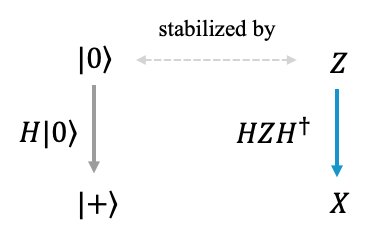
\includegraphics[width=0.3\textwidth]{figures/isomorphism.png}
    \caption{state transformation and generator transformation}
    \label{fig:relation}
\end{figure}

이 방식이 강력한 이유는 qubit의 개수가 증가할 때 진가를 발휘한다. $n$ qubit에 대한 $H^{\otimes n}$연산의 결과를 표현하기 위해서는 $2^n$개의 amplitude를 저장해야하지만 이를 generator로 나타내게 되면 $n$개의 element만 필요로 한다. ($\ket0^{\otimes n}$: stabilized by $\langle Z_1,\cdots,Z_n \rangle$ $\rightarrow$ $\ket +^{\otimes n}$: stabilized by $\langle X_1,\cdots,X_n \rangle$)

$H$ gate말고도 다양한 unitary gate들이 이러한 관계를 이용할 수 있다. Fig.~\ref{fig:relation}에 나와있듯이 CNOT, H, S, P gate들은 모두 pauli group에 가해져서 pauli group을 보존한다. 이러한 역할을 하는 $U$의 집합을 $G_n$의 normalizer라고 부른다. 그중에서도 특히 Pauli group의 normalizer를 \textit{Clifford group}이라고 한다. 
\begin{equation*}
    \forall U \in N(G_n), \qquad UG_nU^\dagger = G_n
\end{equation*}

다양한 gate들이 Clifford group에 속한다는 것을 알 수 있다. 그렇다면, Clifford group에 속하지 않는 gate가 존재할까? Non-Clifford group에 속하는 2가지 중요한 gate는 $\pi/8$ gate (i.e., $T$ gate) 그리고 Toffoli gate이다. 다음과 같이 $T$ gate를 $X$ gate에 가하면 그 결과는 Pauli gate들의 product로 표현할 수 없다.
\begin{equation*}
    T X T^{\dagger}=\frac{X+Y}{\sqrt{2}}
\end{equation*}

그렇다면, Stabilizer formalism을 사용하여 \textbf{measurement}도 표현할 수 있을까? 지금부터는 computational basis에서 measurement를 stabilizer formalism으로 기술하는 방법을 설명하고자한다. 
Pauli observable $g \in G_n$을 측정하다고 하자. 이때, 편의를 위하여 coefficient -1, $\pm i$가 없는 Pauli matrix들의 곱이라고 가정하자. \footnote{$-1$은 결과를 flip하는 것으로 쉽게 구현할 수 있으며 $\pm 1$은 observable은 Hermitian이어야 한다는 조건을 위배하기 때문이다.}
관측을 수행하는 system은 stabilizer $S = \langle g_1, \cdots, g_l \rangle$를 가지는 $\ket \psi$ state에 있다고 하자.\footnote{1dim state: outcome이 2개}

이러한 상황에서는 다음과 같은 2가지 case가 존재한다.
\begin{itemize}
    \item $g$와 $\forall g' \in \langle g_1, \cdots, g_l \rangle$이 commute이다.
    \item $g$와 $\exists g' \in \langle g_1, \cdots, g_l \rangle$이 anti-commute이다. ($g_1$이 anti-commute인 generator라고 하자.)
\end{itemize}
$g$는 Pauli operator들의 product이므로 eigenvalue $\pm 1$을 가지므로 이 observable을 측정한 outcome은 $\pm 1$이며, 그 때 사용하는 measurement operator(projector)는 다음과 같다.
\begin{equation*}
    +1\ :\ \frac{I+g}{2},\qquad -1\ :\ \frac{I-g}{2}
\end{equation*}

\begin{figure}[h]
    \centering
    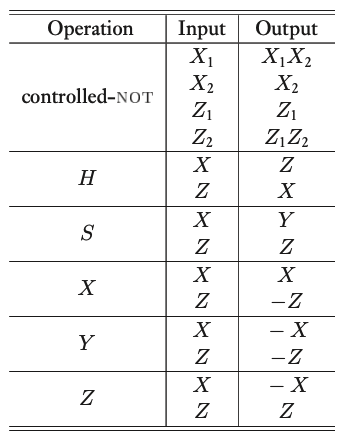
\includegraphics[width=0.38\textwidth]{figures/stabilizer.png}
    \caption{Stabilizer generators transformation}
    \label{fig:transformation}
\end{figure}

먼저 첫 번째 case일 때, measurement를 분석해보자. 임의의 generator $g_i$에 대해서 $g$기 commute하기 때문에 다음이 성립하는데 $g_i$는 $g \ket \psi$를 stabilize하고 $\ket \psi$는 $g$에 의해 stabilize되므로 $g \ket \psi \in V_S$이기 때문에 $\pm g \in S$이다. 
\begin{equation*}
    g_i g \ket \psi = g g_i \ket \psi = g \ket \psi
\end{equation*}
따라서 이를 이용하면, $\ket \psi$에 대한 observable $g$의 관측 확률은 다음과 같다. 
\begin{align*}
    g \ &: \ p(1)=1 ; \quad p(-1)=0 \\
    -g \ &: \ p(1) = 0 ; \quad p(-1) = 1
\end{align*}
또한 measurement operator가 단순히 state를 $V_S$로 projection하는 것이기 때문에 post-measurement state도 변하지 않는다.

그렇다면, 두 번쨰 case에서는 어떻게 될까? Outcome probability는 다음과 같다.
\begin{itemize}
    \item Eq.~\eqref{eq:stabilzer-measure-1}: $g\ket \psi = \ket \psi$ 그리고 $g, g_1$는 anti-commute임을 이용
    \item Eq.~\eqref{eq:stabilizer-measure-2}: Trace의 cyclic property, $g_1 = g_1^\dagger$\footnote{$g_1^2 = \pm I$인데 $-I \notin S$이므로}임을 이용
\end{itemize}
\begin{align}
    p(+1)&= \operatorname{Tr}\left[\frac{I+g}{2}|\psi\rangle\langle\psi|\right] = \operatorname{Tr}\left[\frac{I+g}{2} g_1|\psi\rangle\langle\psi|\right]=\operatorname{Tr}\left[g_1 \frac{I-g}{2}|\psi\rangle\langle\psi|\right] \label{eq:stabilzer-measure-1}\\
    &=\operatorname{Tr}\left[\frac{I-g}{2}|\psi\rangle\langle\psi| g_1\right] = \operatorname{Tr}\left[\frac{I-g}{2}|\psi\rangle\langle\psi| g_1^\dagger\right]\label{eq:stabilizer-measure-2}\\
    &=\operatorname{Tr}\left[\frac{I-g}{2}|\psi\rangle\langle\psi|\right]=p(-1),\label{eq:stabilizer-measure-3}
\end{align}
$p(+1) = p(-1) = 1$이므로 $p(+1) = p(-1) = 1/2$이라고 추정할 수 있다. Post-measurement state는 각각 다음과 같고 각 상태는 새로운 stabilizer $\langle g, g_2, \cdots, g_l \rangle$, $\langle -g, g_2, \cdots, g_l \rangle$을 가진다.
\begin{equation*}
    +1\ :\ \frac{I+g}{\sqrt 2}\ket \psi,\qquad -1\ :\ \frac{I-g}{\sqrt 2} \ket \psi
\end{equation*}


\subsection{Gottesman-Knill theorem}
Stabilizer formalism을 사용할 때, quantum computer의 연산 능력에 대해 한 가지 놀라운 정리를 얻을 수 있다. 이 정리는 quantum computation class의 강력함이 얼마나 애매한지를 보여준다 (...)
\begin{theorem}[Gottesman-Knill theorem]
    다음의 과정을 거치는 quantum circuit은 \textbf{classical computer로 polynomial time에 simulation} 할 수 있다.
    \begin{enumerate}
        \item prepare $\ket 0 ^{\otimes n}$ (in computational basis)
        \item apply unitary gates in \textit{Clifford group}
        \item measure in computational basis (include conditioned on the outcome of measurement)
    \end{enumerate}
\end{theorem}

\lecture{23}{9 Dec. 10:30}{}
\subsection{Stabilizer code constructions}
이제 다시 우리의 원래 주제로 돌아와서 stabilizer formalism을 사용하여 어떻게 QEC를 만들지 생각해보자.

$[n, k]$ stabilizer code $C(S)$는 $G_n$의 subgroup $S$에 의해 stabilize되는 \textbf{vector space} $V_S$로 정의된다.\footnote{$S$는 $-I \notin S$이고 $n-k$개의 independent, commute인 generator를 가진다고 가정.} (i.e., $C(S) \triangleq V_S$)
이때, $S$는 앞에서 가정했던 것처럼 $(1)$ $-I \not \in S$이고 $(2)$ $n-k$개의 linearly independent and commute인 generator $S = \langle g_1, \cdots, g_{n-k} \rangle$를 가진다는 것이다. 

그렇다면 stabilizer code는 어떤 \textit{logical basis state}를 사용할까? Vector space $V_S$의 $2^k$개의 orthonormal basis vector를 선택하여 사용할 수도 있지만, 실제로는 이보다 더 체계적인 방식을 사용한다.
\begin{enumerate}
    \item $\bar{Z_1}, \cdots, \bar{Z_k} \in G_n$\footnote{$\bar{Z_k}$는 logical gate로 $k$번쨰 logical qubit으로 인코딩된 physical qubit에 모두 $Z$ gate를 적용한다.}을 선택하여 $g_1, \cdots, g_{n-k}, \bar{Z_1}, \cdots, \bar{Z_k}$가 서로 linearly independent, commute한 원소를 갖는 집합을 생성하도록 한다.
    \item 따라서 logical qubit $\ket{x_1, \cdots, x_k}_L$은 다음의 stabilizer를 갖는 state로 정의할 수 있다.
    \begin{equation*}
        \left\langle g_1, \cdots, g_{n-k},(-1)^{x_1} \bar{Z}_1, \cdots,(-1)^{x_k} \bar{Z}_k\right\rangle .
    \end{equation*}
\end{enumerate}

그럼 stabilizer code에서 발생하는 error는 무엇일까? $E \in G_n$에 대해 3가지 종류의 에러가 존재한다.
\begin{itemize}
    \item $E$ anti-commute with an element in generator : anti-commute이므로 에러가 발생하면 codeword의 vector space와 orthogonal한 subspace로 mapping되기 때문에 error가 발생했음을 확인하기도 쉽고 쉽게 해결할 수 있다. (e.g., if $E$ is anti-commute with $g_1$, then $Eg_{1}E^\dagger = -g_{1}$\footnote{observable $g_1$을 측정한 결과가 $-1$이므로 오류가 발생했다는 것을 쉽게 알 수 있다.})
    \item $E \in S$ : stabilizer의 성질덕분에 $E \ket \psi = \ket \psi$이므로 오류가 발생하지 않는다.
    \item $E$ commute with \textbf{all} element in generator, but $E \notin S$ : 에러가 발생하면 codeword의 vector space 공간에 존재하는 \textbf{다른 codeword}로 mapping되기 때문에 가장 까다로운 오류이다.
\end{itemize}

$S$의 모든 원소와 commute인 원소 $\E \in G_n$들의 집합을 \textit{centralizer}, $Z(S)$라고 한다. 이때, $Z(S) - S$로 표현되는 집합이 공집합이 아니기 때문에 3번째 type에 해당하는 에러가 발생할 수 있는 것이다. (이때 stabilizer에 대한 centralizer는 stabilizer의 normalizer, $N(S)$와 동일하다. Normalizer는 $S$의 모든 원소에 대해 $EgE^\dagger \in S$가 되도록 하는 원소 $E \in G_n$들의 집합이다.)

\begin{figure}[h]
    \centering
    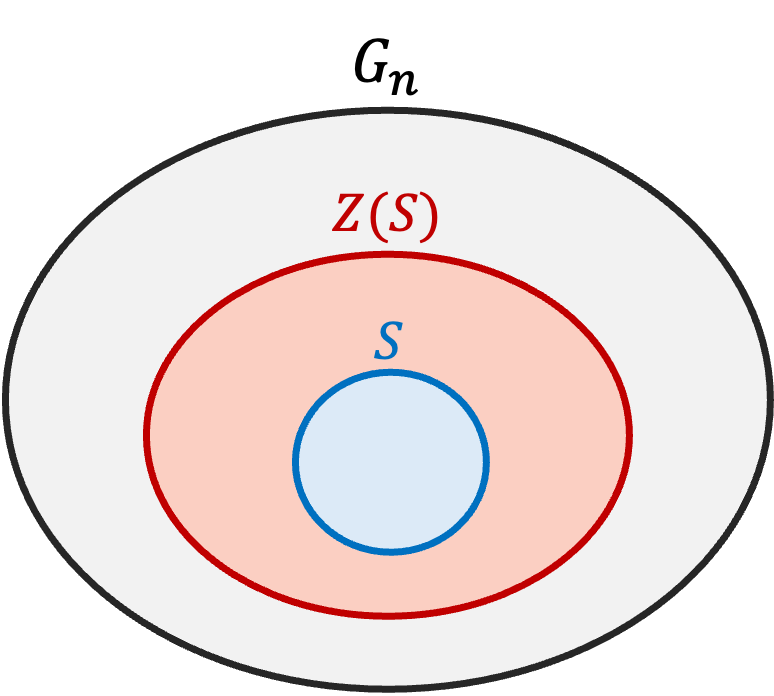
\includegraphics[width=0.35\textwidth]{figures/C7_error_class.png}
    \caption{Error classes}
\end{figure}

\pagebreak

이러한 다양한 에러들의 종류에 대해, stabilizer code에서 QEC condition은 다음과 같이 정리된다.
\begin{theorem}[Error correction conditions for stabilizer codes]
    Let $S$ be the stabilizer for a stabilizer code $C(S)$. Suppose $\{E_j\}$ is a set of operators in $G_n$ such that $E^\dagger_jE_k \not \in N(S) - S$ for all $j$ and $k$.
    Then $\{E_j\}$ is a correctable set of errors for the code $C(S)$. \\
    $\rightarrow$ 즉, 집합 $N(S) - S$에 속하지 않는 원소는 stabilizer code를 사용하여 정정될 수 있다.
\end{theorem}
\begin{proof}
    증명에 앞서, 먼저 original QEC condition이 다음과 같이 정의됨을 기억하자.
    \begin{remark}
        \begin{equation}
            PE_j^\dagger E_k P = \alpha_{ij} P \label{eq:QEC}
        \end{equation}
        where $\alpha_{ij}$ is a Hermitian matrix and $P$ is a projector onto code space (e.g., $C(S)$)
    \end{remark}
    우리가 관찰한 stabilizer code 에러의 3가지 종류에 따르면, $E_j^\dagger E_k \in N(S) - S$에 속하는 에러는 $(1) E_j^\dagger E_k \in S$ 또는 $(2) E_j^\dagger D_k \in G_n - N(S)$이다.
    \vspace{0.2cm}

    먼저 첫 번째 에러에 대해 $P$는 code space에 대한 projector이므로 $S$의 원소에 의해 stabilize된다. 따라서 $E_j^\dagger, E_k$가 $S$의 원소이므로 $PE_j^\dagger E_kP = P$의 관계를 성립한다. $\alpha_{ij} = 1$일 때 Eq.~\eqref{eq:QEC}를 만족한다. 
    반면, 두 번째 에러는 normalizer $N(S)$의 원소가 아니기 때문에 적어도 하나의 generator와는 anti-commute하다. 이 원소를 $g_1$이라고 하자. $\langle g_1, \cdots, g_{n-k}\rangle$이 $S$의 generator set이면, projector $P$를 다음과 같이 쓸 수 있다. 
    \begin{equation*}
        P=\frac{\prod_{l=1}^{n-k}\left(I+g_l\right)}{2^{n-k}}
    \end{equation*}
    $E^\dagger_j g_1 E_k = -g_1$임을 이용하면 $E^\dagger_j E_k$를 가한 상태는 다음과 같다. 
    \begin{equation}
        E_j^{\dagger} E_k P=\left(I-g_1\right) E_j^{\dagger} E_k \frac{\prod_{l=2}^{n-k}\left(I+g_l\right)}{2^{n-k}} \label{eq:proof-1}
    \end{equation}
    이때, Eq.~\eqref{eq:proof-1}는 $(I-g_1)$이 곱해져있고 반대로 $P$는 $(I+g_1)$이 곱해져있는데, $(I+g_1)(I-g_1) = I- g_1^2 = 0$\footnote{Pauli group은 $g_i^2 = I$이므로?}이므로 $PE_j^\dagger E_kP = 0$의 관계를 성립한다. $\alpha_{ij} = 0$일 때 Eq.~\eqref{eq:QEC}를 만족한다.
    \vspace{0.2cm}

    따라서 어떤 종류의 에러이든지 $E_j^\dagger E_k \in G_n - N(S)$라면 QEC condition을 만족하기 때문에 오류정정이 가능하다.
\end{proof}

그렇다면, (정정가능한) 에러가 발생했을때, stabilizer code는 이를 어떻게 감지하고 정정하는가?\\
$\langle g_1, \ldots, g_{n-k} \rangle$가 $S$의 generator이고 $\{E_j\}$가 정정가능한 에러들의 집합이라고 하자. 오류감지를 위하여 generator; observable을 차례대로 측정한 결과로 error syndrome $\beta_1, \beta_2, \cdots, \beta{n-k}$를 얻을 수 있다. 
에러 $E_j$가 발생했을 경우 error syndrome은 $+1, \cdots, \beta_j, \cdots, 1$로 표현된다. 이는 $E_j g_l E_j^\dagger = \beta_l g_l$를 만족한다.
그럼 해당 error syndrome에 대한 복구연산자 $E_j^\dagger$를 적용하여 정정할 수 있다. 

이때 동일한 error syndrome을 가지는 서로 다른 에러 $E_j, E_{j'}$가 존재할 수도 있다. 하지만 이는 에러를 발생시킨 연산자가 무엇이든 관계없이 $E_j^\dagger$나 $E_{j'}^{\dagger}$를 가하여 정정할 수 있다. (by $E_j^\dagger E_{j'} P E_{j'}^\dagger E_j = P $)

\vspace{0.2cm}
Stabilizer code에서도 classical code \textit{distance}를 정의하는 방법과 거의 유사한 방식으로 distance를 정의할 수 있다. 에러 $E \in G_n$ 의 가중치(weight)는 non-trivial한 Pauli matrix의 수로 정의된다.\footnote{자명한 Pauli matrix는 $I$를 이야기한다. $I$는 가해지더라도 오류정정을 할 필요가 없기 때문이다.} 예를 들어,  $X_1Z_4Y_8$ 의 가중치는 3이다.
$C(S)$ 의 거리는  $N(S) - S$에 있는 에러에 대한 minimum distance로 정의된다. $C(S)$가 $[n, k, d]$ 코드이고  $d \geq 2t + 1$ 이라면, 최대 $t$ 큐비트에서 발생하는 오류를 정정할 수 있다.

\subsection{Examples}
\subsubsection{The three qubit bit flip code}
앞에서 다루었던 repetition-three qubit code에 대한 예시를 살펴보자. 이 코드는 $\ket{000}, \ket{111}$을 basis state로 가지기 때문에 logical code space는 stabilizer $S = \langle Z_1Z_2, Z_2Z_3\rangle$을 가진다. 
Bit-flip error 집합 $\{I, X_1, X_2, X_3\}$에 대해, three qubit bit flip code는 두 원소끼리 가능한 모든 product\footnote{e.g., $X_1X_2 \in \{E_j\}$, but $X_1X_2X_3 \notin \{E_j\}$}로 정의되는 집합의 에러를 모두 정정할 수 있다. 이는 $\{E_j\}$에 속한 모든 오류가 $S$의 generator인 $Z_1Z_2, Z_2Z_3$ 둘 중 하나와 반드시 anti-commute하기 때문이다.

\subsubsection{The nine qubit Shor code}
Shor code의 code space에 대한 8개의 generator는 Fig.~\ref{fig:shor_generator}에 나와있다. 이를 이용하면 발생할 수 있는 다양한 에러에 대해서, generator의 원소와 anti-commute인지 아닌지를 확인하는 것만으로 이 code가 해당 오류를 정정할 수 있는지를 분석할 수 있다. (e.g., $X_1Y_4$는 $Z_1Z_2$와 anti-commute이므로 정정가능한 오류)
\begin{figure}[h]
    \centering
    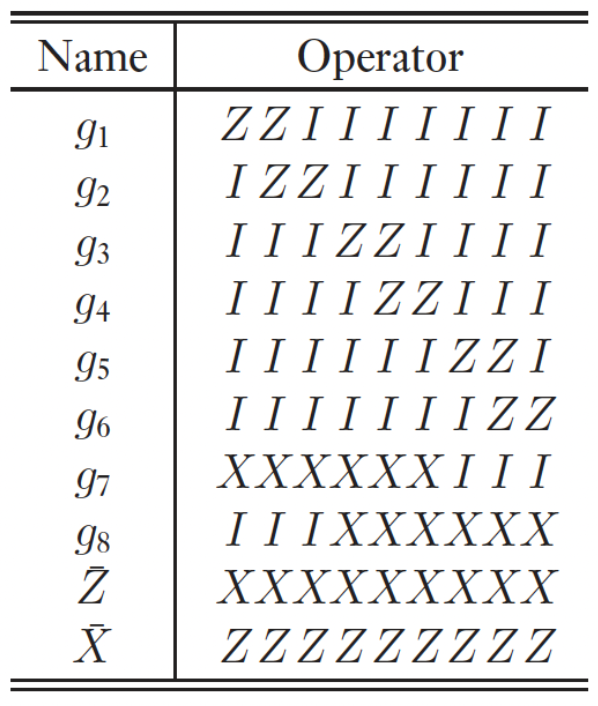
\includegraphics[width=0.25\textwidth]{figures/C7_stabilizer_shor_code.png}
    \caption{generator for Shor code (and logical Z and X)}
    \label{fig:shor_generator}
\end{figure}

\subsubsection{The five qubit code}
에러 정정을 위해서 encoding을 사용할 때, single qubit error를 감지하고 정정할 수 있게하는 logical qubit의 가장 작은 크기는 \textbf{5 qubit}이다. Five qubit code에 대한 stabilizer 역시 Fig.~\ref{fig:five_generator}에 나와있으며, 모든 single qubit error가 five qubit code의 generator와 anti-commute한다는 사실을 쉽게 파악할 수 있다. 
\begin{figure}[h]
    \centering
    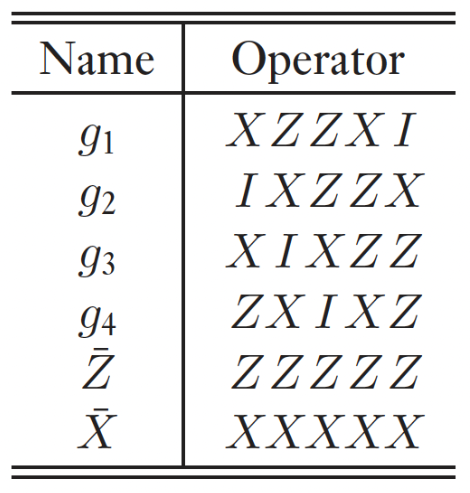
\includegraphics[width=0.2\textwidth]{figures/C7_stabilizer_five_qubit.png}
    \caption{generator for five qubit code (and logical Z and X)}
    \label{fig:five_generator}
\end{figure}

\subsubsection{CSS codes and the seven qubit code}
앞에서 다루었듯이, CSS code는 $C_2 \subset C_1$인 classical linear code $C_1, C_2$를 이용한다. 이 code에 대해서 다음과 같은 check matrix를 정의할 수 있다.\footnote{각 행이 generator, 각 column이 qubit을 의미하며 왼쪽은 Z, 오른쪽은 X를 나타내기 위해 사용된다.}
이 행렬이 stabilizer code를 정의한다는 것을 보이기 위해서는 $H(C_2^\perp)H(C_1)^T = 0$을 만족한다는 것을 확인해야하지만 $C_2 \subset C_1$ 관계 떄문에 $H(C_2^\perp)H(C_1)^T = [H(C_1)G(C_2)]^T 0$가 된다.
\begin{equation*}
    \left(\begin{array}{cc}
        H\left(C_2^{\perp}\right) & 0 \\
        0 & H\left(C_1\right)
    \end{array}\right)
\end{equation*}
CSS code의 한 종류인 Steane code의 경우에는 다음과 같은 logical $Z, X$ gate를 사용한다. 

\begin{equation*}
    \bar{Z} \equiv Z_1 Z_2 \cdots Z_7 ; \quad \bar{X} \equiv X_1 X_2 \cdots X_7 .
\end{equation*}
% \begin{figure}[h]
%     \centering
%     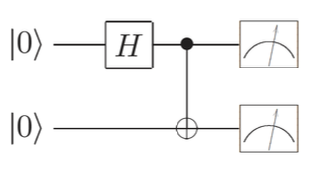
\includegraphics[width=0.22\textwidth]{figures/C7_CNOT.png}
% \end{figure}

\subsection{Quantum circuits for encoding, decoding, and correction}
Stabilizer code의 특징 중 하나는 encoding, decoding, error correction 절차를 잘 구성할 수 있다는 점이다. $[n, k]$ stabilizer code $C(S)$가 generator $\langle g_1, \cdots, g_k\rangle$와 logical gate $\bar Z_1, \cdots, \bar Z_k$를 가질 때, 전체 과정을 나타내보자.
\begin{enumerate}
    \item (encode) logical $\ket{0}_L$ state를 준비 : physical initial state $\ket{0}^{\otimes n}$에 대해서 $n-k$개의 generator, 그리고 $k$개의 logical operator를 측정하면 측정결과에 따라, 적절한 Pauli operator를 가하여 logical init state를 만들 수 있다. 정정하기전의 state는 다음과 같은 stabilizer를 가진다.
    \begin{equation*}
        \left\langle \pm g_1, \ldots, \pm g_{n-k}, \pm Z_1, \ldots, \pm Z_k\right\rangle
    \end{equation*}
    \item (decode) QC에서는 logical state를 측정한 결과로부터 기존의 값(decode)을 알 수 있기 때문에, decoding 과정이 별도로 필요하지 않다. 
    \item (measurement) generator나 logical Pauli gate; observable을 측정하기 위해서 Fig.~\ref{fig:measurement}와 같은 회로를 구성한다. 이는 $M$에 대한 \textbf{eigenvalue}를 측정한다는 의미로 해석할 수 있다. Pauli group $G_n$에 속한 원소들은 모두 $\pm 1$의 eigenvalue를 가진다.
\end{enumerate}
\begin{figure}[h]
    \centering
    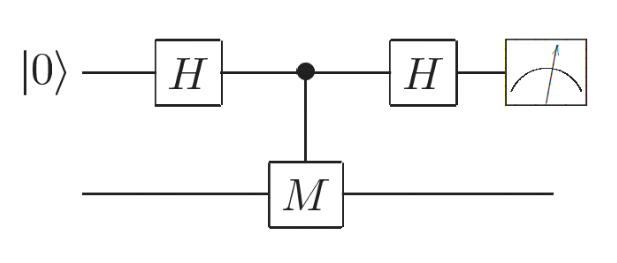
\includegraphics[width=0.3\textwidth]{figures/C7_measurement.png}
    \caption{Measurement observable}
    \label{fig:measurement}
\end{figure}
\begin{figure}[h]
    \centering
    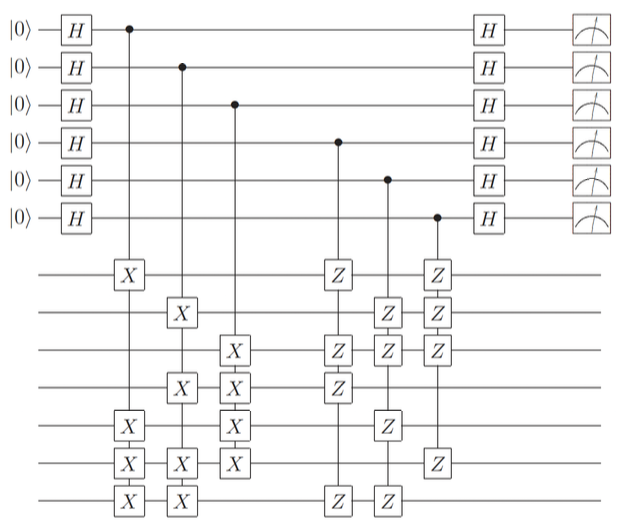
\includegraphics[width=0.6\textwidth]{figures/C7_stean_code_measurement.png}
    \caption{Stean code measurement}
\end{figure}

\lecture{24}{11 Dec. 10:30}{}
\section{Fault-tolerant quantum computation}
지금까지 우리는 QEC에서 진행되는 절차가 모두 \textit{noiseless}라는 이상적인 가정에서 QEC가 가능하다는 것을 주장했었다. 그러나, 실제 quantum computer는 여전히 noise가 존재하고 이로인하여 QEC 과정에서도 오류가 발생할 수 있다. 
그렇다면 실제 device에서는 QEC가 불가능할까? 놀랍게도, 1개의 gate를 가할 때 오류가 발생할 확률인 $p$가 특정 \textit{threshold}보다 작은경우 arbitrary long quantum circuit도 작은 오류확률을 가지며 효율적으로 수행할 수 있다는 사실이 알려져있다. 

\subsection{Fault-tolerance: the big picture}

Fault-tolerance quantum computation은 각 연산을 적용할 때마다 에러가 발생할 가능성을 고려하면서도 안정적인 연산을 수행할 수 있도록 하는 방법이다. 
이 섹션에서는 양자 컴퓨터에서 \textit{error propagation}, 그리고 \textit{error accumulate}가 왜 fault-tolerance에 문제가 되는지에 대해서 설명한 뒤, 
fault-tolerant가 어떻게 구현되는지를 예시로 들고자한다. 마지막으로 \textbf{concatenation}을 통해 어떤 arbitrary long quantum circuit도 신뢰성있게 실행할 수 있다는 threshold theorem에 대해서 설명하려고 한다.

\subsubsection{Fundamental issues}
Fault-tolerance computation을 위해서 $(1)$ QEC code로 인코딩된 logical qubit을 이용하며, $(2)$ 각 quantum \textit{logical} gate가 적용될때마다 error correction을 실시하는 단순한 아이디어를 생각해볼 수 있다. (See Fig.~\ref{fig:FT-circui}) 그러나 이런 방법으로도 충분하지 않다. 다음의 2가지 문제점이 존재한다.
\begin{itemize}
    \item Logical (encoded) gate는 \textit{error propagation}을 야기시킬 수 있다. 예를 들어, CNOT gate라면 control qubit가 가지고 있던 오류가 target qubit에도 전달된다.
    \item QEC에서 수행하는 error correction procedure 자체가 faulty 할 수 있다.
\end{itemize}
따라서 Fault-tolerant quantum computation을 위해서는, encoded gate를 잘 설계해야하낟. 

\begin{figure}[h]
    \centering
    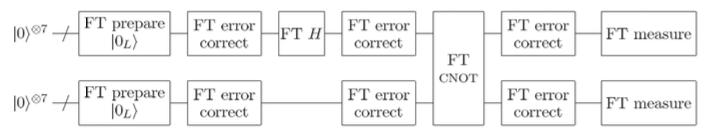
\includegraphics[width=0.75\textwidth]{figures/C7_FT_gate.png}
    \caption{Fault-tolerance circuit}
    \label{fig:FT-circui}
\end{figure}

\subsubsection{Fault-tolerant operations: definitions}
Fault-tolerance computation을 구현하기에 앞서, Fault-tolerance의 기준이 무엇인지를 정의하고자한다.
\begin{definition}[Fault-tolerance]
    If only one component in the procedure fails then the failure cases \textit{at most} \textbf{one error in each encoded block} of qubits output from the procedure.
\end{definition}
즉, 어떤 procedure\footnote{e.g., encoded gate를 구현하는 procedure}가 fault-tolerance하다고 이야기하기 위해서는 그 procedure를 이루는 각 component(e.g., gate, measurement, state preparation, ...)에 오류가 발생하였더라도 procedure가 끝났을 때 output logical qubit안에는 최대 1개의 에러만이 발생해야한다. 이러한 single qubit error는 우리가 앞에서 소개했던 매커니즘을 이용하여 충분히 오류정정을 수행할 수 있다.

특히 fault-tolerant measurement도 이러한 특성을 만족해야하는데, 만약 procedure를 이루는 각 component의 에러 확률중에서 가장 높은 값이 $p$일 때, 측정 결과는 $O(p^2)$의 오류확률을 가져야한다. 

본 강의에서는 단순화를 위하여 Pauli-error $\{I, X, Y, Z\}$에 대해서만 고려한다. 예를 들어, $X_1$ 오류가 있는 상태에서 CNOT을 하면 $C(X)X_1I = C(X)X_1C(X)^\dagger C(X) = X_1X_2C(X)$가 된다. 즉, CNOT이 올바르게 적용되었지만 bit flip error가 다른 qubit으로 전파되었다.

\subsubsection{Example: fault-tolerant CNOT}
본격적으로 fault-tolerant CNOT을 구현하는 procedure에 대해서 분석해보자. Fig.~\ref{fig:cnot-detail}에서 표현한 것처럼 FT CNOT은 4가지의 component를 가진다. 각 component에 오류가 발생하더라도 encoded qubit안에서 2개 이상의 오류가 발생할 확률이 $O(p^2)$가 된다는 것을 보이려고 한다. 

\begin{itemize}
    \item 각 logical qubit에 단일 에러가 존재하는 경우 : CNOT을 통과하면서 첫 번째 logical qubit에 존재하던 에러가 두 번쨰 logical qubit으로 전파되면서 두 번쨰 logical에 두 개의 오류를 유발할 수 있다. 만약 이전 단계의 회로들이 모두 FT로 설계되었다면, 각 logical qubit에 단일 에러가 발생할 확률은 $c_0p$ 이하이다.\footnote{$c_0$은 오류가 발생할 수 있는 위치를 나타내는 상수} 두 logical qubit에 에러가 독립적으로 발생한다고 가정하면, CNOT 통과이후 단일 logical qubit에서 2개 이상의 에러를 가질 확률은 $c_0^2p^2$ 이하이다.
    \item 하나의 logical qubit에 단일 에러가 존재하고 CNOT에서 추가로 단일 에러가 발생하는 경우 :\\ 이 에러 이벤트의 발생확률은 $c_1 p^2$이다.
    \item CNOT에서 2개의 에러가 발생하는 경우
    \item CNOT에서 단일 에러가 발생하고 syndrome measurement를 수행하면서 추가로 단일 에러가 발생하는 경우
    \item etc ...
\end{itemize}

FT CNOT procedure에서 발생할 수 있는 모든 error event에 대해서 logical qubit에 두 개 이상의 에러가 발생할 확률은 모두 $cp^2$이하 이다. 따라서, FT CNOT을 구현하는 회로의 각 구성 요소가 $p$ 확률로 에러를 발생시킬 수 있어도 FT CNOT은 $1 - cp^2$ 확률로 성공한다.

\begin{figure}[h]
    \centering
    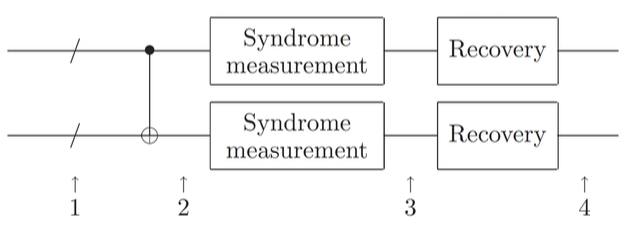
\includegraphics[width=0.45\textwidth]{figures/C7_FT_CNOT_high.png}
    \caption{Fault-tolerant CNOT procedure}
    \label{fig:cnot-detail}
\end{figure}

\subsubsection{Concatenated codes and the threshold theorem}
앞에서 보인 FT CNOT은 기존의 성공확률에 비해서 더 높은 성공확률을 보이기는 하지만, 여전히 그렇게까지 강력해보이지는 않는다. 이를 위해서 한 가지 강력한 아이디어를 도입하고자한다.

아이디어는 FT procedure를 \textbf{recursively} 반복하는 것이다. 예를 들어, Fig.~\ref{fig:concat}에서 사용하는 two-level concatenation을 분석해보자.
회로를 이루는 component에 대해 physical error probability가 $p$일 때, 첫 번째 encoding을 통해서 logical error rate $cp^2$을 얻을 수 있다. 그 다음으로 logical qubit $\ket{0}_{L_1}$을 physical qubit으로 생각하고 두 번쨰 encoding을 도입할 수 있다. (e.g., $\ket{0}_{L_2} = \ket{0_{L_1}0_{L_1}0_{L_1}}$)
따라서 error rate $p_1 \triangle cp^2$에 대하여, 두 번쨰 encoding을 통해서 얻을 수 있는 error rate는 $p_2 \triangleq c (cp^2)^2 = c^3p^4$이다. 
이를 반복하면 $k$-level concatenation을 통해서 $(cp)^{2^k}/ c$ error rate를 얻을 수 있다. $k$-level concatenation을 위해 필요한 cost(size of simulating circuit)는 original circuit size의 $d^k$배 이다. 이때, $d$는 FT procedure를 위해 필요한 maximum number of operations을 의미한다. 

Original circuit size가 problem size $n$에 대해 polynomial size (i.e., $p(n)$)를 가질 때, target accuracy $\epsilon$을 달성하기 위해서 필요한 반복횟수 $k$는 얼마일까? Target accuracy를 달성하기 위해서는, 회로를 이루는 각각의 gate에 대한 target accuracy가 $\epsilon/p(n)$이라는 것을 쉽게 알 수 있다. 따라서, $k$-concatenation FT gate에 대해서 다음을 만족해서 target accuracy를 달성할 수 있을 것이다.
\begin{equation*}
    \frac{(c p)^{2^k}}{c} \leq \frac{\epsilon}{p(n)} .
\end{equation*}
이떄, physical error $p < p_{\text{thresh}} \triangle 1/c$의 조건을 만족하면 $k\rightarrow \infty$에 따라서 우리가 원하는 임의의 정확도를 얻을 수 있다.\footnote{만약 $p = p_{\text{thresh}}$라면 $k$가 증가하더라도 $(cp)^{2^k}/c$가 constant가 되기 때문에 target error를 달성할 수 없다.}
그렇다면, target accuracy를 달성하기 위해 필요한 circuit의 크기는 얼마일까? $d^k$에 위의 관계식으로부터 얻은 $k$를 대입하면 다음을 얻을 수 있고
\begin{equation*}
    d^k=O(\operatorname{poly}(\log p(n) / \epsilon)),
\end{equation*}
원본 회로의 크기가 $p(n)$이므로 FT simulate circuit의 size는 다음과 같다.
\begin{equation*}
    O(\operatorname{poly}(\log p(n) / \epsilon) p(n))
\end{equation*}
이를 \textit{threshold theorem}이라고 한다. 

\begin{figure}[h]
    \centering
    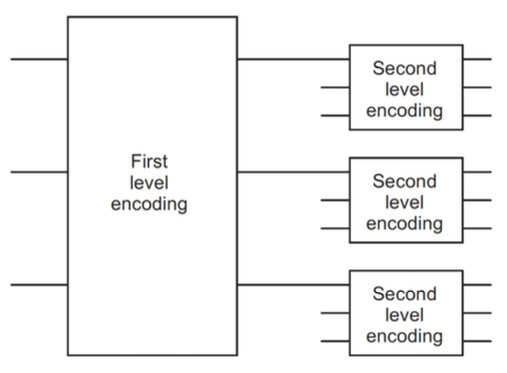
\includegraphics[width=0.4\textwidth]{figures/C7_FT_concatenation.png}
    \caption{Concatenation}
    \label{fig:concat}
\end{figure}

\subsection{Fault-tolerant quantum logic gate}
우리는 $\{H, S, CNOT, T\}$ gate가 universal gate set이라는 사실을 이미 알고있다. 따라서 Fault-tolerant $H, S, CNOT$ 그리고 $T$ gate를 구현할 수 있으면\footnote{여기서 이야기하는 FT는 Fig.~\ref{fig:cnot-detail}와 같은 전체 과정이 아니라 이 과정의 구성요소인, FT CNOT을 의미한다.} Fault-tolerant gate procedure를 구축할 수 있고 이를 이용하여 Fault-tolerant computation을 수행할 수 있다.

\subsubsection{Normalizer operations}
$\{H, S, CNOT\}$ gate는 Clifford group에 속하는 게이트이기 때문에 쉽게 구현할 수 있다. Stean code에서 사용하는 logical gate는 다음과 같이 정의된다.
\begin{equation*}
    \bar{Z}=Z_1 Z_2 \cdots Z_7 ; \quad \bar{X}=X_1 X_2 \cdots X_7.
\end{equation*}
즉, logical gate를 구현하기 위해서는 단순히 logical qubit을 이루는 각각의 physical qubit에 \textit{single qubit gate}를 가하면 된다. 
각 gate는 하나의 qubit에만 작용하기 때문에, error propagation이 일어나지 않는다. 따라서 logical gate를 구현하기 위해서 physical operation을 각 qubit에 서로 \textbf{individually} 적용하면 그 logical gate는 fault-tolerant 하다는 사실을 알 수 있다. (\textit{transversality property})
\begin{theorem}[Easten-Knill theorem]
    No quantum error correcting code can transversely implement a universal gate set.
\end{theorem}

마찬가지로 CNOT gate 역시 transversality property를 가지도록 구현할 수 있다. Control qubit으로 사용되는 logical qubit에 있는 \textbf{모든} physical qubit과 target qubit으로 사용되는 logical qubit에 있는 \textbf{모든} physical block을 CNOT gate로 연결한다.
이 연산은 동일한 block안에서 서로 연결되지 않기 때문에 독립적으로 동작하기 때문에 fault-tolerance하다. 
\begin{figure}[h]
    \centering
    \[
        \begin{array}{c}
        \Qcircuit @C=1.0em @R=0.8em {
            & \qw & \ctrl{3} & \qw      & \qw & \qw \\
            & \qw & \qw      & \ctrl{3} & \qw  & \qw \\
            & \qw & \qw      & \qw      & \ctrl{3} & \qw \inputgroupv{1}{3}{.8em}{.8em}{\ket{\psi}_L}\\ 
            & \qw & \targ    & \qw      & \qw & \qw \\
            & \qw & \qw & \targ & \qw & \qw \\
            & \qw & \qw & \qw & \targ & \qw \inputgroupv{4}{6}{.8em}{.8em}{\ket{\psi}_L}
        }
        \end{array}
        \]
    \caption{Logical CNOT gate} \label{fig:locial-CNOT-circuit}
\end{figure}

\subsubsection{Fault-tolerent $\pi/8$ gate}
반면, $T$ gate의 구현은 앞선 방식들과는 다른 방법을 따른다. 이 과정은 (1) 특정한 magic state $\ket{\Theta}$로 state preparation을 수행한 뒤, 앞에서 이미 구현한 FT normalizer operation들을 이용하여 회로를 구성한다.
\begin{enumerate}
    \item initial state : $\ket{\theta}\ket{\psi}$. FT T gate는 첫 번쨰 qubit에 $T\ket{\psi}$를 저장하는 방식으로 동작한다. 
    \begin{equation*}
        |\Theta\rangle=\frac{|0\rangle+e^{i \pi / 4}|1\rangle}{\sqrt{2}} .
    \end{equation*}    
    \item apply FT CNOT : 다음을 얻는다.
    \begin{equation*}
        \frac{1}{\sqrt{2}}\left[|0\rangle(a|0\rangle+b|1\rangle)+e^{i \pi / 4}|1\rangle(a|1\rangle+b|0\rangle)\right]=\frac{1}{\sqrt{2}}\left[\left(a|0\rangle+b e^{i \pi / 4}|1\rangle\right)|0\rangle+\left(b|0\rangle+a e^{i \pi / 4}|1\rangle\right)|1\rangle\right]
    \end{equation*}
    \item measure second qubit : 두 번째 qubit의 측정 결과가 $0$일 때는 post-state가 우리가 원하는 $T \ket{\psi}$이므로 측정 결과가 $1$일 때만 추가적인 정정을 필요로한다.
    \item if outcome is $1$, then apply $SX$
    \begin{equation*}
        S X=\left(\begin{array}{ll}
            1 & 0 \\
            0 & i
            \end{array}\right)\left(\begin{array}{ll}
            0 & 1 \\
            1 & 0
            \end{array}\right)
    \end{equation*}
    $SX$를 가하면 우리가 원하는 state를 얻을 수 있다. 
    \begin{equation*}
        a|0\rangle+b e^{i \pi / 4}|1\rangle .
    \end{equation*}    
\end{enumerate}
그렇다면, initial state $\ket{\Theta}$는 어떻게 생성할 수 있을까? \textit{Measurement} outcome이 그 observable에 해당하는 eigenvalue를 반환하는 것이라는 걸 기억하자.
$\ket{0}$가 $+1$을 eigenvalue로 가지는 $Z$의 eigenvector이고 $\ket{\Theta}$가 $+1$을 eigenvalue로 가지는 $e^{-i\pi/4}SX$의 eigenvector라는 사실을 이용하자.

따라서 Clifford group의 특징을 이용하면, $Z \rightarrow HZH^\dagger \rightarrow THZH^\dagger T^\dagger = e^{-i\pi/4} SX$이므로 이를 이용하여 $\ket{0} \rightarrow H\ket 0 \rightarrow TH \ket 0 = \ket \Theta$임을 알 수 있다. 따라서 $H, T$ gate를 차례대로 가함으로서 $\Theta$ 상태를 만들 수 있다.
단, 이 과정은 \textbf{faulty}를 허용하지 않는 방법이다.\footnote{fault-tolerance T gate를 모르는데 T gate를 사용함} 따라서 대신 $e^{-i \pi/4} SX$로 $\ket 0$을 \textbf{측정}함으로서 $\Theta$ state를 준비할 수 있다. 한 가지 주의해야할 점은 $HT$ gate를 적용한 뒤 측정결과가 $-1$이라면, $Z$ gate를 가하여 $\ket \Theta$로 변환해야한다.
\begin{align*}
    e^{-i \pi/4} SX \ket{\Theta'} = - \ket{\Theta'},\\
    \Rightarrow e^{-i \pi/4} SX \left(Z\ket{\Theta'}\right) =  \left(Z\ket{\Theta'}\right) = \ket{\Theta}
\end{align*}
\begin{figure}[h]
    \centering
    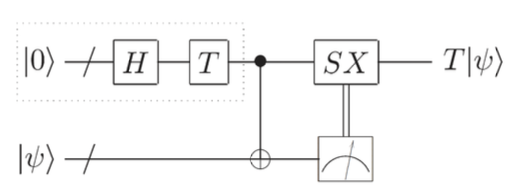
\includegraphics[width=0.38\textwidth]{figures/C7_FT_T.png}
    \caption{Fault-tolerance T gate}
\end{figure}

\subsubsection{Fault-tolerant measurement}
그렇다면, 마지막으로 fault-tolerance measurement는 어떻게 구현할 수 있을까? Measurement는 QEC에서 syndrome measurement를 진행할 때나, state preparation을 위해서, 또는 실제 quantum circuit의 마지막 연산 단게에서 결과를 확인하기 위해 사용될 수도 있다.
따라서 FT measurement를 구현하는 것은 quantum computing에서 매우 중요한 단계라고 말할 수 있다. 

다음 그림은 일반적은 measurement gate를 나타낸다. 이처럼 measurement 단계에서 controlled operation을 사용하여 QEC에 필요한 정보를 수집하기 때문에 첫 번째 qubit $\ket 0$에서 발생한 에러가 다른 qubit에 모두 전파될 수 있다. 
\begin{figure}[h]
    \centering
    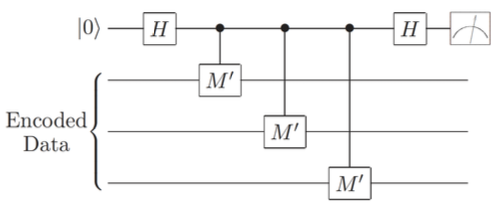
\includegraphics[width=0.45\textwidth]{figures/C7_QEC_measurement.png}
    \caption{Measurement}
\end{figure}

Three qubit encoded code에서의 fault-tolerance measurement는 Fig.~\ref{fig:FT-measure}에 나와있다.
\begin{enumerate}
    \item prepare : 관측을 위해 사용되는 ancilla qubit을 \textit{cat-state} $\ket {00 \cdots 0} + \ket{11 \cdots 1}$로 준비시킨다. prepare step은 FT가 아니기 떄문에, 앞에서 수행한 회로가 제대로 된 연산을 수행했는지 검증하는 단계를 필요로한다.\footnote{왜 $H^n$으로 안하지...?}
    \item verify : 주어진 ancilla qubit이 cat state인지 확인하기 위해서 모든 qubit들의 combination에 대해 두 qubit이 동일한 parity를 가지는지를 측정한다. ($Z_iZ_j$)
    \item controlled-M : $M$의 eigenvalue를 측정하기 위해서 ancilla qubit와 data qubit 사이에 1-to-1 controlled $M$을 가한다.
    \item decode : 측정을 위해 decode를 수행한다.
\end{enumerate}

\begin{figure}[h]
    \centering
    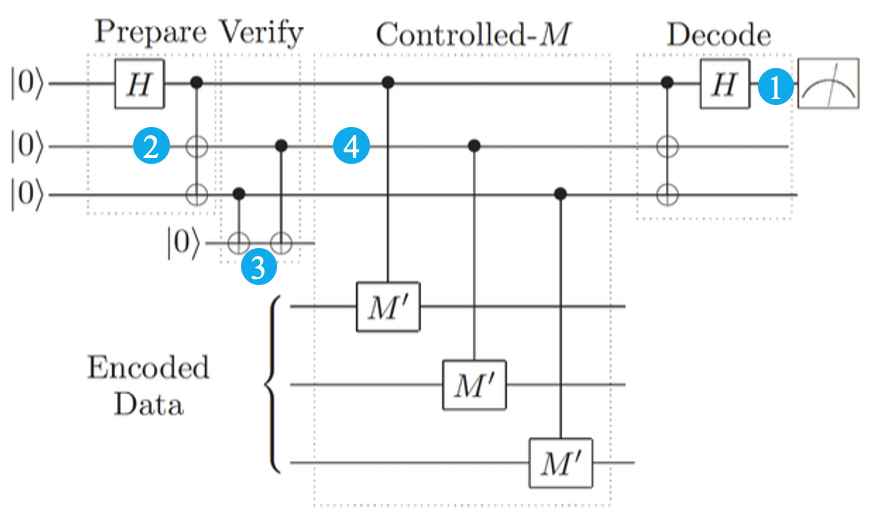
\includegraphics[width=0.6\textwidth]{figures/C7_FT_measurement.png}
    \caption{Fault-tolerance measurement}
    \label{fig:FT-measure}
\end{figure}

이 과정을 따르는 measurement가 왜 fault-tolerance한지 각 component에 에러가 발생했을 경우에 따라 분석해보자.
\begin{enumerate}[(1)]
    \item decode 이후에 오류가 발생 : 측정 과정을 3번 반복하여, 과반수를 얻은 결과를 택한다. 이 경우 측정이 잘못될 확률은 최대 $O(p^2)$이 된다.\footnote{encoded data로 연결되지 않기 때문에 데이터 손상은 없다.} (\textit{majority vote})
    \item prepare 과정에서 오류가 발생 : verify 과정에서 오류가 발생했다는 사실을 확인할 수 있으므로 정정할 수 있다.
    \item verify 과정에서 오류가 발생 : 오류가 있는 ancilla qubit을 이용하면 $Z$ error의 경우 encoded data를 변경시키지 않지만, $X, Y$는 encoded data에 오류를 일으킬 수 있다.\\
    $\rightarrow$ $Z$ error는 majority vote로 해결할 수 있으며, $X, Y$와 같은 single qubit error는 QEC를 통해서 충분히 정정될 수 있다.
    \item controlled-M을 수행할 때 오류가 발생 : (3)에서 이야기 한 것처럼 오류가 전파되어 encoded data를 손상시킬 수 있지만, 이는 single qubit error이고 QEC로 정정될 수 있다. 
\end{enumerate}

\begin{figure}[h]
    \centering
    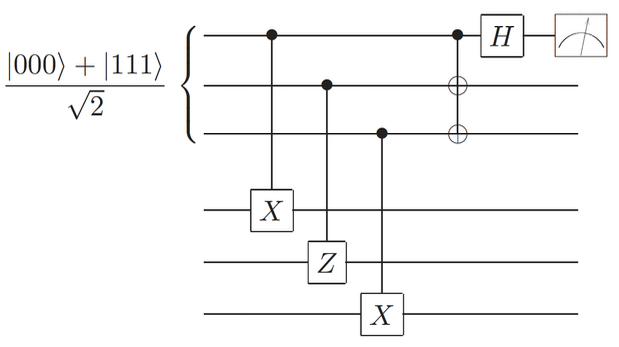
\includegraphics[width=0.45\textwidth]{figures/C7_FT_stabilizer.png}
    \caption{Stabilizer measurement}
\end{figure}
